\documentclass[11pt,a4paper]{article}

\usepackage[margin=2.2cm]{geometry}
\usepackage[T1]{fontenc}
\IfFileExists{lmodern.sty}{\usepackage{lmodern}}{}
\usepackage{amsmath,amssymb}
\usepackage{booktabs}
\usepackage{float}
\usepackage{array}
\newcolumntype{L}[1]{>{\raggedright\arraybackslash}p{#1}}
\usepackage{enumitem}
\usepackage{xcolor}
\usepackage{listings}
\usepackage{tikz}
\usetikzlibrary{arrows.meta,positioning,calc,shapes.geometric,fit,decorations.pathreplacing}
\usepackage[most]{tcolorbox}
\usepackage[colorlinks=true,linkcolor=blue!50!black,urlcolor=blue!50!black]{hyperref}
\usepackage{fancyhdr}

\setlength{\parindent}{0pt}
\setlength{\emergencystretch}{2em}
\setlength{\parskip}{6pt}
\renewcommand{\arraystretch}{1.25}

\pagestyle{fancy}
\fancyhf{}
\lhead{\small Compiler Design -- Intermediate Code Generation}
\rhead{\small SDD \& SDT}
\cfoot{\thepage}

% ---------- Boxes ----------
\newtcolorbox{defbox}[1]{colback=blue!4,colframe=blue!55!black,fonttitle=\bfseries,title={#1},breakable}
\newtcolorbox{examplebox}[1]{colback=green!4,colframe=green!45!black,fonttitle=\bfseries,title={#1},breakable}
\newtcolorbox{notebox}[1]{colback=orange!6,colframe=orange!75!black,fonttitle=\bfseries,title={#1},breakable}
\newtcolorbox{pitfallbox}[1]{colback=red!5,colframe=red!60!black,fonttitle=\bfseries,title={#1},breakable}

% ---------- Macros ----------
\newcommand{\kw}[1]{\textbf{#1}}
\newcommand{\gen}[1]{\ensuremath{\mathbf{gen}(#1)}}
\newcommand{\cc}{\mathbin{\|}}
\newcommand{\at}[2]{\ensuremath{#1.\mathit{#2}}}
\newcommand{\tok}[1]{\ensuremath{\mathtt{#1}}}
\newcommand{\lbl}[1]{\ensuremath{\mathbf{label}(#1)}}
\newcommand{\goto}{\kw{goto}}

\lstdefinestyle{tac}{
  basicstyle=\ttfamily\small,
  frame=single,
  backgroundcolor=\color{gray!8},
  rulecolor=\color{gray!60},
  columns=fullflexible,
  keepspaces=true,
  xleftmargin=4pt,
  xrightmargin=4pt,
  aboveskip=4pt,
  belowskip=4pt
}
\lstset{style=tac}

\title{\textbf{Intermediate Code Generation\\[2pt] using Syntax-Directed Definitions (SDD) \\ and Syntax-Directed Translation (SDT)}\\[6pt]
\large Lecture Notes based on \emph{Compilers: Principles, Techniques, and Tools} (the ``Dragon Book''),\\ 2nd Edition, Aho, Lam, Sethi, Ullman -- Chapters 5 and 6}
\author{}
\date{}

\begin{document}
\maketitle
\thispagestyle{fancy}

\begin{tcolorbox}[colback=gray!5,colframe=gray!50,title=\textbf{Suggested Lecture Plan (3--4 lectures)}]
\begin{description}[leftmargin=2.2cm,style=nextline]
\item[Lecture 1] Role of intermediate code; forms of IR: syntax trees, DAGs, three-address code, quadruples, triples, indirect triples.
\item[Lecture 2] \emph{Syntax-directed definitions and translation, from scratch:} why syntax alone is not enough, attributes, semantic rules, synthesized and inherited attributes, dependency graphs, S- and L-attributed definitions; then SDTs: actions inside productions, postfix translation, marker nonterminals.
\item[Lecture 3] Translation of expressions and assignments, array references, type checking and conversion.
\item[Lecture 4] Boolean expressions and short-circuit code, flow-of-control statements, backpatching, switch statements and procedure calls; revision and exercises.
\end{description}
\end{tcolorbox}

\tableofcontents
\newpage

%====================================================================
\section{Introduction: Why Intermediate Code?}
%====================================================================

In the \emph{analysis--synthesis} model of a compiler, the \textbf{front end} analyses the source program and produces an \textbf{intermediate representation (IR)}; the \textbf{back end} synthesises the target program from that IR.

\begin{figure}[htbp]
\centering
\resizebox{\textwidth}{!}{%
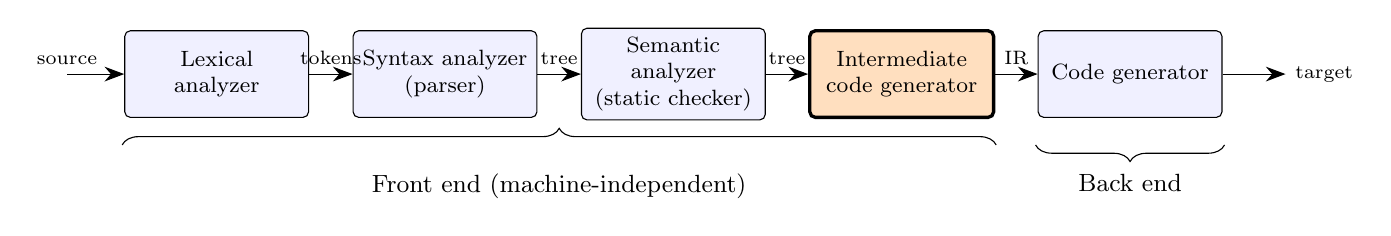
\begin{tikzpicture}[
  box/.style={draw,rounded corners=2pt,minimum height=1.1cm,minimum width=2.3cm,text width=2.1cm,align=center,font=\footnotesize,fill=blue!6},
  ir/.style={draw,rounded corners=2pt,minimum height=1.1cm,minimum width=2.3cm,text width=2.1cm,align=center,font=\footnotesize,fill=orange!25,very thick},
  arr/.style={-{Stealth[length=2.5mm]}}]
 \node[box] (lex) at (0,0) {Lexical analyzer};
 \node[box] (par) at (2.9,0) {Syntax analyzer (parser)};
 \node[box] (sem) at (5.8,0) {Semantic analyzer (static checker)};
 \node[ir]  (icg) at (8.7,0) {Intermediate code generator};
 \node[box] (cg)  at (11.6,0) {Code generator};
 \draw[arr] (-1.9,0)--(lex.west) node[pos=0,above,font=\scriptsize]{source};
 \draw[arr] (lex)--(par) node[midway,above,font=\scriptsize]{tokens};
 \draw[arr] (par)--(sem) node[midway,above,font=\scriptsize]{tree};
 \draw[arr] (sem)--(icg) node[midway,above,font=\scriptsize]{tree};
 \draw[arr] (icg)--(cg) node[midway,above,font=\scriptsize]{IR};
 \draw[arr] (cg.east)--++(0.8,0) node[right,font=\scriptsize]{target};
 \draw[decorate,decoration={brace,amplitude=6pt}] (-1.2,-0.9)--(9.9,-0.9) node[midway,below=7pt,font=\small]{Front end (machine-independent)};
 \draw[decorate,decoration={brace,amplitude=6pt}] (12.8,-0.9)--(10.4,-0.9) node[midway,below=7pt,font=\small]{Back end};
\end{tikzpicture}}
\caption{Position of the intermediate code generator in a compiler. The shaded (thick) box is the topic of these notes. In practice, static checking and intermediate code generation are often done together in one pass.}
\end{figure}

\subsection{Advantages of using an intermediate representation}
\begin{itemize}
\item \textbf{Retargeting.} A compiler for $m$ languages and $n$ machines needs only $m$ front ends plus $n$ back ends ($m+n$ pieces instead of $m \times n$ separate compilers) if they share one IR. For example, 3 languages and 4 machines need $3+4=7$ pieces instead of $12$ compilers.
\item \textbf{Machine-independent optimisation.} Optimisations (common sub-expression elimination, constant folding, loop-invariant code motion, ...) are applied once on the IR.
\item \textbf{Simplicity.} Complex source constructs are lowered to a few simple operations, making code generation easier.
\end{itemize}

\begin{notebox}{Static checking vs.\ intermediate code}
Static checking includes type checking and syntactic checks that the grammar cannot enforce (e.g., \texttt{break} must be inside a loop). Dragon Book Chapter 6 treats type checking and intermediate-code generation together, because both are done by attaching attributes and actions to the grammar.
\end{notebox}

%====================================================================
\section{Variants of Syntax Trees and Intermediate Representations}
%====================================================================

\subsection{Syntax trees (abstract syntax trees)}
\label{sec:syntaxtree}
A \textbf{syntax tree} is a condensed form of the parse tree: operators and keywords appear as \emph{interior nodes}, and operands as children. Chains of single productions (such as $E\to T\to F\to\mathbf{id}$) disappear, and so do punctuation tokens such as parentheses. The tree keeps only what later phases need: \emph{which operation is applied to which operands}.

\begin{examplebox}{Example: parse tree vs.\ syntax tree for $a + b * c$}
Take the usual grammar $E \to E + T \mid T$, \ $T \to T * F \mid F$, \ $F \to \mathbf{id}$.

\begin{figure}[H]
\centering
\begin{tikzpicture}[
  n/.style={inner sep=1.5pt,font=\small},
  s/.style={circle,draw,minimum size=6.5mm,inner sep=0pt,font=\small}]
 \node[n] (E0) at (0,0) {$E$};
 \node[n] (E1) at (-2.2,-1) {$E$};
 \node[n] (pl) at (0,-1) {$+$};
 \node[n] (T1) at (2.2,-1) {$T$};
 \node[n] (T2) at (-2.2,-2) {$T$};
 \node[n] (F1) at (-2.2,-3) {$F$};
 \node[n] (ia) at (-2.2,-4) {\textbf{id}$_a$};
 \node[n] (T3) at (1.4,-2) {$T$};
 \node[n] (st) at (2.4,-2) {$*$};
 \node[n] (F3) at (3.4,-2) {$F$};
 \node[n] (F2) at (1.4,-3) {$F$};
 \node[n] (ib) at (1.4,-4) {\textbf{id}$_b$};
 \node[n] (ic) at (3.4,-3) {\textbf{id}$_c$};
 \foreach \a/\b in {E0/E1,E0/pl,E0/T1,E1/T2,T2/F1,F1/ia,T1/T3,T1/st,T1/F3,T3/F2,F2/ib,F3/ic}
   \draw[gray] (\a)--(\b);
 \node[font=\small] at (0.6,-5) {(a) parse tree: 13 nodes};
 \begin{scope}[xshift=7.5cm]
  \node[s] (P) at (0,0) {$+$};
  \node[s] (A) at (-1.2,-1.2) {$a$};
  \node[s] (M) at (1.2,-1.2) {$*$};
  \node[s] (B) at (0.2,-2.4) {$b$};
  \node[s] (C) at (2.2,-2.4) {$c$};
  \foreach \a/\b in {P/A,P/M,M/B,M/C} \draw (\a)--(\b);
  \node[font=\small] at (1,-5) {(b) syntax tree: 5 nodes};
 \end{scope}
\end{tikzpicture}
\caption{Parse tree and syntax tree of $a+b*c$. Precedence survives in the shape of the syntax tree: $*$ is below $+$, so it is evaluated first.}
\end{figure}

Most parse-tree nodes only record \emph{how the grammar was written} (the chains $E\to T\to F$); the syntax tree has 5 nodes. Parentheses never appear in a syntax tree: $(a+b)*c$ simply has the $+$ node below the $*$ node.
\end{examplebox}

\subsection{Directed acyclic graphs (DAGs) for expressions}
A \textbf{DAG} identifies the \emph{common sub-expressions}: a node is shared if the same sub-expression appears more than once. It shows the same information as a syntax tree but is more compact, and it directly suggests how to generate efficient code that computes a common sub-expression only once.

\begin{examplebox}{Example: tree vs.\ DAG for $a + a*(b-c) + (b-c)*d$}
Figure~\ref{fig:treedag} shows the syntax tree (left) and the DAG (right). In the DAG, the leaf $a$ and the sub-expression $b-c$ are each shared by two parents.

\textbf{Why arrows?} A DAG is a \emph{directed} acyclic graph. Each edge points from an operator node to one of its operands (``this operation uses that value''), so a node with two incoming arrows is a value that is used twice. There is no cycle because an expression can never be an operand of itself. In a tree the direction is the same but is left implicit, since every node has exactly one parent.

\begin{figure}[H]
\centering
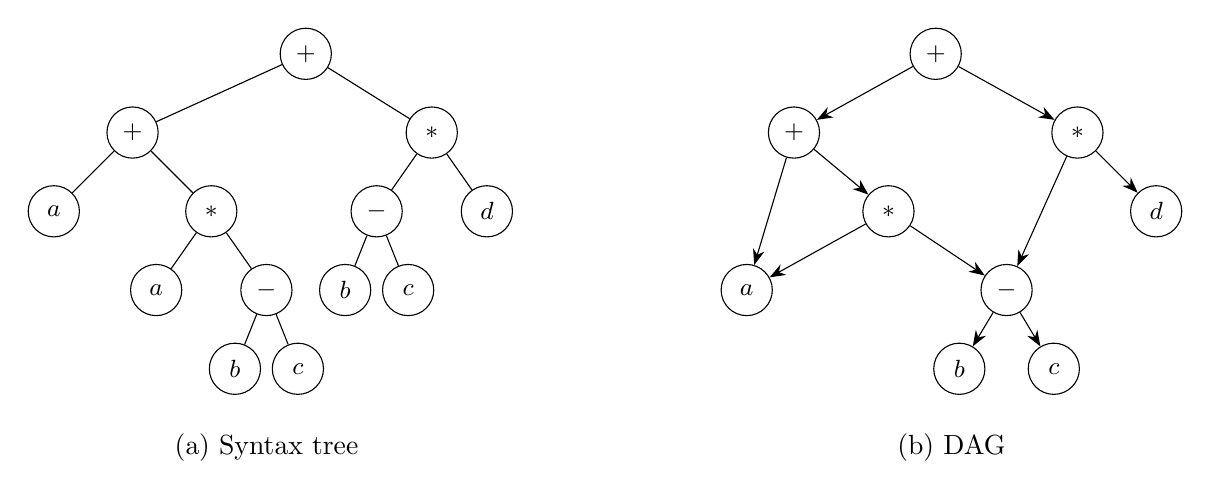
\begin{tikzpicture}[
  n/.style={circle,draw,minimum size=6.5mm,inner sep=0pt,font=\small},
  sibling distance=0pt]
 % ---- syntax tree ----
 \node[n] (r) at (0,0) {$+$};
 \node[n] (l) at (-2.2,-1) {$+$};
 \node[n] (rm) at (1.6,-1) {$*$};
 \node[n] (a1) at (-3.2,-2) {$a$};
 \node[n] (lm) at (-1.2,-2) {$*$};
 \node[n] (a2) at (-1.9,-3) {$a$};
 \node[n] (m1) at (-0.5,-3) {$-$};
 \node[n] (b1) at (-0.9,-4) {$b$};
 \node[n] (c1) at (-0.1,-4) {$c$};
 \node[n] (m2) at (0.9,-2) {$-$};
 \node[n] (d)  at (2.3,-2) {$d$};
 \node[n] (b2) at (0.5,-3) {$b$};
 \node[n] (c2) at (1.3,-3) {$c$};
 \draw (r)--(l); \draw (r)--(rm);
 \draw (l)--(a1); \draw (l)--(lm);
 \draw (lm)--(a2); \draw (lm)--(m1);
 \draw (m1)--(b1); \draw (m1)--(c1);
 \draw (rm)--(m2); \draw (rm)--(d);
 \draw (m2)--(b2); \draw (m2)--(c2);
 \node at (-0.5,-5) {(a) Syntax tree};
 % ---- DAG ----
 \begin{scope}[xshift=8cm]
 \node[n] (R) at (0,0) {$+$};
 \node[n] (L) at (-1.8,-1) {$+$};
 \node[n] (RM) at (1.8,-1) {$*$};
 \node[n] (LM) at (-0.6,-2) {$*$};
 \node[n] (A) at (-2.4,-3) {$a$};
 \node[n] (M) at (0.9,-3) {$-$};
 \node[n] (B) at (0.3,-4) {$b$};
 \node[n] (C) at (1.5,-4) {$c$};
 \node[n] (D) at (2.8,-2) {$d$};
 \begin{scope}[every path/.style={-{Stealth[length=2mm]}}]
 \draw (R)--(L); \draw (R)--(RM);
 \draw (L)--(A); \draw (L)--(LM);
 \draw (LM)--(A); \draw (LM)--(M);
 \draw (RM)--(M); \draw (RM)--(D);
 \draw (M)--(B); \draw (M)--(C);
 \end{scope}
 \node at (0.2,-5) {(b) DAG};
 \end{scope}
\end{tikzpicture}
\caption{Syntax tree and DAG for $a + a*(b-c) + (b-c)*d$. In the DAG every edge is an arrow from an operator to one of its operands.}
\label{fig:treedag}
\end{figure}
\end{examplebox}

\subsubsection{The value-number method for constructing DAGs}
\label{sec:vn}
\textbf{The problem.} While building the tree for an expression, we want to \emph{reuse} a node if the same sub-expression has already been built. To do this we need a fast way to answer: ``Have I already created a node for $b - c$?'' The \textbf{value-number method} gives a simple answer. Here we assume the \emph{syntax tree} of the expression has already been built (Figure~\ref{fig:treedag}(a)). We convert it into a DAG by visiting the tree nodes in \textbf{post-order} (left subtree, right subtree, then the node itself), so that the children of a node are always handled before the node.

\textbf{The idea.} Keep all nodes in an \textbf{array of records}. Each record describes one node of the DAG, and the \emph{position (index) of the record in the array is the node's value number}. The value number is therefore just the node's \emph{name}: ``node 4'' means ``the record at position 4''.

\begin{defbox}{What the numbers mean}
\begin{itemize}
\item \textbf{Value number} = the index of a record in the array = the identity of one DAG node. It is \emph{not} the numeric value of the expression (the number 4 does not mean the expression evaluates to 4).
\item A \textbf{leaf record} stores the kind of leaf and what it is: $(\mathbf{id},\ \text{pointer to symbol-table entry})$ for a variable, or $(\mathbf{num},\ \text{value})$ for a constant.
\item An \textbf{interior record} has the form $(\mathit{op},\ \mathit{left},\ \mathit{right})$. Here $\mathit{op}$ is the operator, and \textbf{\textit{left} and \textit{right} are the value numbers of the two child nodes}, i.e., they are \emph{pointers} to other records (the operands).
\end{itemize}
\end{defbox}

\textbf{Example.} The record $(*,\ 1,\ 4)$ means: ``a node for the operator $*$ whose left child is node~1 and whose right child is node~4''. Looking up the array, node 1 is the leaf $a$ and node 4 is $b - c$; so this record stands for $a * (b - c)$.

\begin{defbox}{Algorithm: finding or creating a node}
To create a node with signature $\langle \mathit{op},\ l,\ r\rangle$ (where $l$ and $r$ are value numbers of the children that were already created):
\begin{enumerate}[nosep]
\item \textbf{Search} the array for a record with exactly the same $\mathit{op}$, $\mathit{left}=l$, and $\mathit{right}=r$.
\item If such a record \textbf{exists}, do not create anything; \textbf{return its value number}. (This is the common sub-expression being shared.)
\item Otherwise \textbf{append} a new record $(\mathit{op},\ l,\ r)$ at the end of the array and \textbf{return its index} as the new value number.
\end{enumerate}
(For speed, a hash table keyed on $(\mathit{op},l,r)$ replaces the linear search in step 1.)
\end{defbox}

\textbf{Why does comparing only $(\mathit{op},l,r)$ work?} Two nodes represent the same expression exactly when they have the same operator and the same children. Children are the same exactly when they have the same value numbers (because every distinct sub-expression gets exactly one number). So, by building from the leaves upward, equal sub-expressions always get equal numbers.

\begin{examplebox}{A second example: $(a+b)*(a+b)$ and the commutativity trap}
Post-order requests and the records they create:
\begin{enumerate}[nosep]
\item leaf $a$ $\Rightarrow$ new record 1; \ leaf $b$ $\Rightarrow$ new record 2; \ $\langle +,1,2\rangle$ $\Rightarrow$ new record 3.
\item Second copy: leaf $a$ $\Rightarrow$ found (1); leaf $b$ $\Rightarrow$ found (2); $\langle +,1,2\rangle$ $\Rightarrow$ \textbf{found (3)}, shared.
\item $\langle *,3,3\rangle$ $\Rightarrow$ new record 4 (both children are the same node).
\end{enumerate}
The DAG has 4 nodes (the tree has 7) and gives \texttt{t1 = a + b}, \texttt{t2 = t1 * t1}. Note that the $*$ node has \emph{two} arrows into the same node: its left and its right operand are one and the same value.

\begin{center}
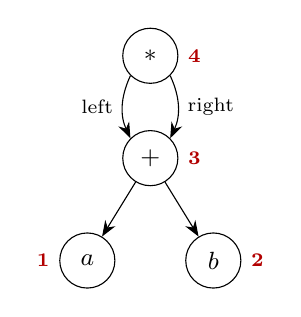
\begin{tikzpicture}[
  n/.style={circle,draw,minimum size=7mm,inner sep=0pt,font=\small},
  tag/.style={font=\scriptsize\bfseries,text=red!70!black},
  ar/.style={-{Stealth[length=2mm]}}]
 \node[n,label={[tag]right:4}] (m) at (0,0) {$*$};
 \node[n,label={[tag]right:3}] (p) at (0,-1.3) {$+$};
 \node[n,label={[tag]left:1}]  (a) at (-0.8,-2.6) {$a$};
 \node[n,label={[tag]right:2}] (b) at (0.8,-2.6) {$b$};
 \draw[ar] (m.south west) to[bend right=25] node[left,font=\scriptsize]{left} (p.north west);
 \draw[ar] (m.south east) to[bend left=25] node[right,font=\scriptsize]{right} (p.north east);
 \draw[ar] (p)--(a); \draw[ar] (p)--(b);
\end{tikzpicture}
\end{center} Now try $(a+b)*(b+a)$: the second sum is $\langle +,2,1\rangle$, which is \emph{not} equal to $\langle +,1,2\rangle$, so a new node is created and $a+b$ is computed twice. To avoid this, a compiler stores the children of a commutative operator in a canonical order (say, smaller value number first); then $\langle +,2,1\rangle$ becomes $\langle +,1,2\rangle$ and is shared.
\end{examplebox}

\begin{pitfallbox}{Limits of the method}
The test ``same $\mathit{op}$ and same children'' finds only \emph{syntactically identical} sub-expressions (up to the operand-order trick above). It does not know that $x*2$ and $x+x$ are equal; that needs algebraic simplification, a separate optimisation.
\end{pitfallbox}

\paragraph{Step-by-step example: $a + a*(b-c) + (b-c)*d$.}
We walk the syntax tree of Figure~\ref{fig:treedag}(a) in post-order: $a$, $a$, $b$, $c$, then $-$, $*$, $+$ of the left part, then $b$, $c$, $-$, $d$, $*$, and finally the root $+$. At every tree node we ask the array for the matching DAG node. Table~\ref{tab:vntrace} shows each request and what the algorithm does.

\begin{table}[H]
\centering
\small
\begin{tabular}{@{}c l l l c@{}}
\toprule
\textbf{Step} & \textbf{Request} & \textbf{Found in array?} & \textbf{Action} & \textbf{Returns} \\ \midrule
1 & leaf $a$ & no & create record 1: $(\mathbf{id}, a)$ & 1 \\
2 & leaf $a$ (2nd time) & \textbf{yes, record 1} & nothing created & 1 \\
3 & leaf $b$ & no & create record 2: $(\mathbf{id}, b)$ & 2 \\
4 & leaf $c$ & no & create record 3: $(\mathbf{id}, c)$ & 3 \\
5 & $\langle -, 2, 3\rangle$ \quad ($b-c$) & no & create record 4: $(-,2,3)$ & 4 \\
6 & $\langle *, 1, 4\rangle$ \quad ($a*(b-c)$) & no & create record 5: $(*,1,4)$ & 5 \\
7 & $\langle +, 1, 5\rangle$ \quad ($a + a*(b-c)$) & no & create record 6: $(+,1,5)$ & 6 \\
8 & leaf $b$ (2nd time) & \textbf{yes, record 2} & nothing created & 2 \\
9 & leaf $c$ (2nd time) & \textbf{yes, record 3} & nothing created & 3 \\
10 & $\langle -, 2, 3\rangle$ \quad ($b-c$ again) & \textbf{yes, record 4} & nothing created -- \emph{shared!} & 4 \\
11 & leaf $d$ & no & create record 7: $(\mathbf{id}, d)$ & 7 \\
12 & $\langle *, 4, 7\rangle$ \quad ($(b-c)*d$) & no & create record 8: $(*,4,7)$ & 8 \\
13 & $\langle +, 6, 8\rangle$ \quad (whole expression) & no & create record 9: $(+,6,8)$ & 9 \\ \bottomrule
\end{tabular}
\caption{Trace of the value-number method. Steps 2, 8, 9, 10 reuse existing nodes; step 10 is where the common sub-expression $b-c$ is detected.}
\label{tab:vntrace}
\end{table}

The result has only $9$ nodes (a plain syntax tree would have $13$: it repeats $a$, $b$, $c$ and the whole $b-c$ sub-tree). The final value number $9$ identifies the root of the DAG.

\begin{figure}[H]
\centering
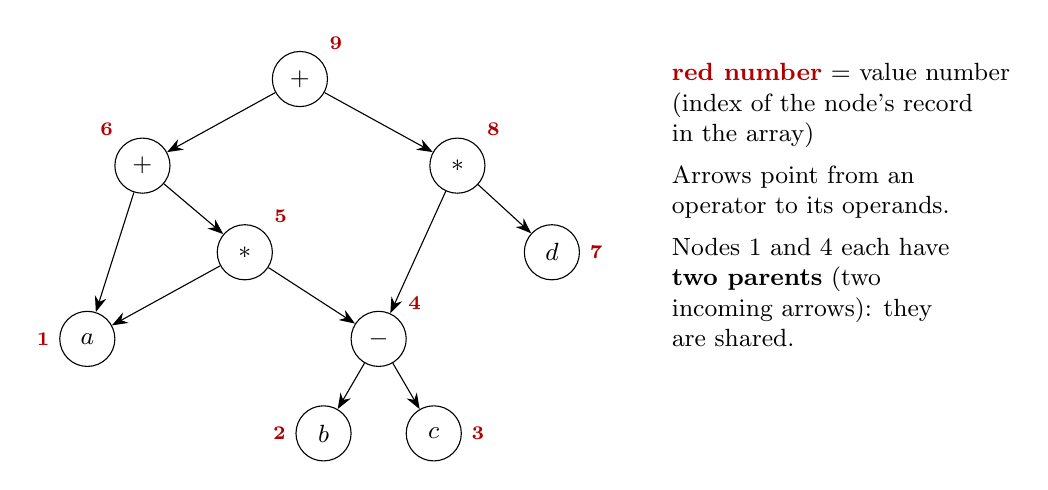
\begin{tikzpicture}[
  n/.style={circle,draw,minimum size=7mm,inner sep=0pt,font=\small},
  tag/.style={font=\scriptsize\bfseries,text=red!70!black}]
 \node[n,label={[tag]above right:9}] (n9) at (0,0) {$+$};
 \node[n,label={[tag]above left:6}]  (n6) at (-2,-1.1) {$+$};
 \node[n,label={[tag]above right:8}] (n8) at (2,-1.1) {$*$};
 \node[n,label={[tag]above right:5}] (n5) at (-0.7,-2.2) {$*$};
 \node[n,label={[tag]left:1}]  (n1) at (-2.7,-3.3) {$a$};
 \node[n,label={[tag]above right:4}] (n4) at (1,-3.3) {$-$};
 \node[n,label={[tag]left:2}]  (n2) at (0.3,-4.5) {$b$};
 \node[n,label={[tag]right:3}] (n3) at (1.7,-4.5) {$c$};
 \node[n,label={[tag]right:7}] (n7) at (3.2,-2.2) {$d$};
 \begin{scope}[every path/.style={-{Stealth[length=2mm]}}]
 \draw (n9)--(n6); \draw (n9)--(n8);
 \draw (n6)--(n1); \draw (n6)--(n5);
 \draw (n5)--(n1); \draw (n5)--(n4);
 \draw (n8)--(n4); \draw (n8)--(n7);
 \draw (n4)--(n2); \draw (n4)--(n3);
 \end{scope}
 \node[font=\small,align=left,anchor=west] at (4.6,-1.6) {\textcolor{red!70!black}{\textbf{red number}} = value number\\(index of the node's record\\in the array)\\[4pt] Arrows point from an\\operator to its operands.\\[4pt] Nodes 1 and 4 each have\\\textbf{two parents} (two\\incoming arrows): they\\are shared.};
\end{tikzpicture}
\caption{The DAG for $a + a*(b-c) + (b-c)*d$ with the value number of every node in red. Arrows go from operator to operand.}
\label{fig:dagvn}
\end{figure}

\begin{figure}[H]
\centering
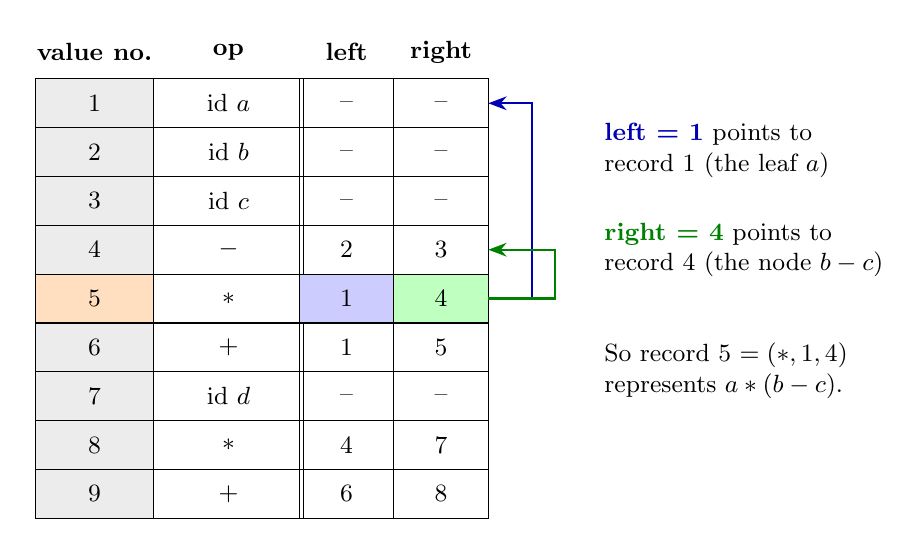
\begin{tikzpicture}[
  c/.style={draw,minimum height=0.62cm,font=\small},
  hd/.style={minimum height=0.62cm,font=\small\bfseries}]
 % header
 \node[hd,minimum width=1.5cm] at (0.75,0.65) {value no.};
 \node[hd,minimum width=1.9cm] at (2.45,0.65) {op};
 \node[hd,minimum width=1.2cm] at (3.95,0.65) {left};
 \node[hd,minimum width=1.2cm] at (5.15,0.65) {right};
 \foreach \i/\op/\l/\r/\y in {
   1/{id $a$}/--/--/0,
   2/{id $b$}/--/--/-0.62,
   3/{id $c$}/--/--/-1.24,
   4/$-$/2/3/-1.86,
   5/$*$/1/4/-2.48,
   6/$+$/1/5/-3.10,
   7/{id $d$}/--/--/-3.72,
   8/$*$/4/7/-4.34,
   9/$+$/6/8/-4.96} {
   \node[c,minimum width=1.5cm,fill=gray!15] (v\i) at (0.75,\y) {\i};
   \node[c,minimum width=1.9cm] (o\i) at (2.45,\y) {\op};
   \node[c,minimum width=1.2cm] (l\i) at (3.95,\y) {\l};
   \node[c,minimum width=1.2cm] (r\i) at (5.15,\y) {\r};
 }
 % highlight record 5
 \node[c,minimum width=1.2cm,fill=blue!20] at (3.95,-2.48) {1};
 \node[c,minimum width=1.2cm,fill=green!25] at (5.15,-2.48) {4};
 \node[c,minimum width=1.5cm,fill=orange!25] at (0.75,-2.48) {5};
 % arrows from record 5 to its children
 \draw[-{Stealth},blue!70!black,thick] (5.75,-2.48) to[bend left=0] (6.3,-2.48) |- (6.3,0) -- (5.75,0);
 \draw[-{Stealth},green!50!black,thick] (5.75,-2.48) -- (6.6,-2.48) |- (6.6,-1.86) -- (5.75,-1.86);
 \node[font=\small,align=left,anchor=west] at (7.1,-0.6) {\textcolor{blue!70!black}{\textbf{left = 1}} points to\\record 1 (the leaf $a$)};
 \node[font=\small,align=left,anchor=west] at (7.1,-1.86) {\textcolor{green!50!black}{\textbf{right = 4}} points to\\record 4 (the node $b-c$)};
 \node[font=\small,align=left,anchor=west] at (7.1,-3.4) {So record 5 $=(*,1,4)$\\represents $a*(b-c)$.};
\end{tikzpicture}
\caption{The array of records after processing the example. Interior records contain \emph{value numbers of their children}; here record 5 refers to records 1 and 4.}
\label{fig:dagarray}
\end{figure}

\paragraph{The whole procedure.} Converting a syntax tree into a DAG is a single post-order traversal:
\begin{lstlisting}
int buildDAG(TreeNode t) {            // returns a value number
    if (t is a leaf)
        return findOrCreateLeaf(t);   // search (id/num, entry); create if absent
    l = buildDAG(t.left);             // children first (post-order)
    r = buildDAG(t.right);
    return findOrCreateNode(t.op, l, r);   // search (op,l,r); create if absent
}
\end{lstlisting}
The ``search'' is only a \emph{lookup of an identical record} in the array (or hash table); it is not a second traversal of the tree.

\begin{notebox}{Looking ahead}
Building the tree first and then converting it is easy to understand. Later, after we study syntax-directed definitions (Section~\ref{sec:sddtree}), we will see that the same DAG can be built \emph{directly while parsing}, without constructing the tree at all: the parser simply calls the find-or-create routine each time it recognises an operator.
\end{notebox}

\subsection{Three-address code (TAC)}
In \textbf{three-address code} every instruction has \emph{at most one operator on the right side} and at most three addresses (two operands and one result). Compound expressions are broken into temporaries, so the order of evaluation is made explicit.

For $a + a*(b-c) + (b-c)*d$ the TAC (from the DAG, reusing $t_1 = b-c$) is:
\begin{lstlisting}
t1 = b - c
t2 = a * t1
t3 = a + t2
t4 = t1 * d
t5 = t3 + t4
\end{lstlisting}
Without the DAG (from the tree) $b-c$ would be computed twice.

\subsubsection{Generating three-address code from a DAG}
\label{sec:dag2tac}
Three-address code can be generated from the DAG alone; no SDD or SDT is needed.

\paragraph{Idea.} Every \emph{interior} node of the DAG becomes exactly \emph{one} three-address instruction, with a fresh temporary holding its result. \emph{Leaves} generate no instruction: they only supply a name (a variable such as $a$, or a constant). A shared node is still one node, so it produces only one instruction; this is how the DAG removes the common sub-expression.

\paragraph{Order.} Process the records of the array in increasing order of value number. A node's children were always created before the node, so their value numbers are smaller, and their results are ready when the node is reached. The array order is therefore already a valid evaluation order.

\begin{lstlisting}
for i = 1 to n:                          // records in the array, in index order
    if record i is a leaf:
        name[i] = the variable or constant it stands for
    else:                                // record i = (op, left, right)
        name[i] = newTemp()
        emit( name[i] = name[left] op name[right] )
\end{lstlisting}
Here $\mathit{name}[i]$ is the address that holds the value of node $i$. For an assignment $x = \langle\text{expression}\rangle$ we finish with one more instruction, \texttt{x = name[root]}.

\begin{table}[H]
\centering
\small
\begin{tabular}{@{}c l c c c l@{}}
\toprule
\textbf{Record} & \textbf{Content} & $\mathit{name}[\mathit{left}]$ & $\mathit{name}[\mathit{right}]$ & $\mathit{name}[i]$ & \textbf{Instruction emitted} \\ \midrule
1 & \texttt{id} $a$ & -- & -- & $a$ & (none, leaf) \\
2 & \texttt{id} $b$ & -- & -- & $b$ & (none, leaf) \\
3 & \texttt{id} $c$ & -- & -- & $c$ & (none, leaf) \\
4 & $(-,2,3)$ & $b$ & $c$ & $t_1$ & \texttt{t1 = b - c} \\
5 & $(*,1,4)$ & $a$ & $t_1$ & $t_2$ & \texttt{t2 = a * t1} \\
6 & $(+,1,5)$ & $a$ & $t_2$ & $t_3$ & \texttt{t3 = a + t2} \\
7 & \texttt{id} $d$ & -- & -- & $d$ & (none, leaf) \\
8 & $(*,4,7)$ & $t_1$ & $d$ & $t_4$ & \texttt{t4 = t1 * d} \\
9 & $(+,6,8)$ & $t_3$ & $t_4$ & $t_5$ & \texttt{t5 = t3 + t4} \\ \bottomrule
\end{tabular}
\caption{Generating three-address code from the array of Figure~\ref{fig:dagarray} (the DAG of $a + a*(b-c) + (b-c)*d$). Node 4 has two parents (nodes 5 and 8) but produces only one instruction; both parents use $t_1$.}
\end{table}

\paragraph{Three ways to obtain three-address code.}
\begin{center}
\small
\begin{tabular}{@{}L{3.6cm} L{4.7cm} L{5.4cm}@{}}
\toprule
\textbf{Method} & \textbf{How} & \textbf{Common sub-expressions} \\ \midrule
1.\ From a finished DAG & Scan the array in index order (above); no SDD/SDT needed. & Computed once (shared nodes). \\
2.\ During DAG construction & Whenever find-or-create \emph{creates} a node, emit its instruction; when it finds an existing node, emit nothing. Needs SDT (Section~\ref{sec:sddtree}). & Computed once. \\
3.\ SDD/SDT directly from the parse (Section~\ref{sec:exprtac}) & Each reduction emits an instruction using \textit{newTemp} and \textit{gen}; no DAG is built. & Computed again each time they occur (e.g., $b-c$ twice). \\ \bottomrule
\end{tabular}
\end{center}
SDD/SDT is the \emph{mechanism} for generating code in one pass while parsing; the DAG is what gives \emph{sharing}. Methods 1 and 2 give the same code.

\begin{notebox}{Caution: assignments inside the DAG}
If the DAG covers several statements and a variable is \emph{reassigned} in between (e.g., \texttt{a = a + 1}), a later use of $a$ is a different value and must not share the old leaf or any node built from it. Compilers handle this by creating a new leaf (a new value number) after each assignment. For single expressions, as in these notes, the issue does not arise.
\end{notebox}


\subsubsection{Addresses and instructions}
An \textbf{address} can be: (i) a \emph{name} (source variable; a pointer to its symbol-table entry), (ii) a \emph{constant}, or (iii) a compiler-generated \emph{temporary}.

\begin{table}[htbp]
\centering
\small
\begin{tabular}{@{}l l@{}}
\toprule
\textbf{Instruction form} & \textbf{Meaning} \\ \midrule
\texttt{x = y op z} & binary assignment \\
\texttt{x = op y} & unary assignment (\texttt{minus}, \texttt{not}, conversions) \\
\texttt{x = y} & copy \\
\texttt{goto L} & unconditional jump \\
\texttt{if x goto L}\ /\ \texttt{ifFalse x goto L} & conditional jump on truth value \\
\texttt{if x relop y goto L} & conditional jump on comparison \\
\texttt{param x}, \texttt{call p, n}, \texttt{y = call p, n}, \texttt{return y} & procedure calls \\
\texttt{x = y[i]}, \texttt{x[i] = y} & indexed copy (memory at address $y + i$) \\
\texttt{x = \&y}, \texttt{x = *y}, \texttt{*x = y} & address and pointer assignments \\
\texttt{L:} & label (a symbolic name for an instruction) \\ \bottomrule
\end{tabular}
\caption{Common three-address instruction forms.}
\end{table}

\subsubsection{Representations of three-address code}
Take the source statement $a = b * -c + b * -c$.

\begin{center}
\begin{minipage}[t]{0.30\textwidth}
\textbf{(a) Three-address code}
\begin{lstlisting}
t1 = minus c
t2 = b * t1
t3 = minus c
t4 = b * t3
t5 = t2 + t4
a  = t5
\end{lstlisting}
\end{minipage}\hfill
\begin{minipage}[t]{0.65\textwidth}
\textbf{(b) Quadruples} -- (op, arg1, arg2, result)

\smallskip
\small
\begin{tabular}{@{}c l l l l@{}}
\toprule
 & op & arg$_1$ & arg$_2$ & result \\ \midrule
0 & \texttt{minus} & c  &    & t1 \\
1 & \texttt{*}     & b  & t1 & t2 \\
2 & \texttt{minus} & c  &    & t3 \\
3 & \texttt{*}     & b  & t3 & t4 \\
4 & \texttt{+}     & t2 & t4 & t5 \\
5 & \texttt{=}     & t5 &    & a  \\ \bottomrule
\end{tabular}
\end{minipage}
\end{center}

\begin{center}
\begin{minipage}[t]{0.47\textwidth}
\textbf{(c) Triples} -- (op, arg1, arg2); a result is referred to by the \emph{position} of its triple.

\smallskip
\small
\begin{tabular}{@{}c l l l@{}}
\toprule
 & op & arg$_1$ & arg$_2$ \\ \midrule
0 & \texttt{minus} & c  &   \\
1 & \texttt{*}     & b  & (0) \\
2 & \texttt{minus} & c  &   \\
3 & \texttt{*}     & b  & (2) \\
4 & \texttt{+}     & (1) & (3) \\
5 & \texttt{=}     & a  & (4) \\ \bottomrule
\end{tabular}
\end{minipage}\hfill
\begin{minipage}[t]{0.47\textwidth}
\textbf{(d) Indirect triples} -- a list of pointers to triples.

\smallskip
\small
\begin{tabular}{@{}c c@{}}
\toprule
 instruction & pointer \\ \midrule
35 & (0) \\ 36 & (1) \\ 37 & (2) \\ 38 & (3) \\ 39 & (4) \\ 40 & (5) \\ \bottomrule
\end{tabular}

\smallskip
\emph{(triples as in (c))}
\end{minipage}
\end{center}

\begin{table}[htbp]
\centering
\small
\begin{tabular}{@{}L{2.6cm} L{5.6cm} L{5.6cm}@{}}
\toprule
 & \textbf{Advantage} & \textbf{Disadvantage} \\ \midrule
Quadruples & Results are named explicitly (temporaries); instructions can be moved freely during optimisation. & Needs extra space for temporaries and symbol-table entries. \\
Triples & No temporaries; more compact. & Moving a triple changes positions, so all references to it must be updated. \\
Indirect triples & Reordering only rearranges the pointer list, so triples keep their positions. & Extra level of indirection; an additional list is needed. \\ \bottomrule
\end{tabular}
\caption{Comparison of the three representations.}
\end{table}

\subsubsection{Static single-assignment (SSA) form -- a brief note}
In \textbf{SSA form} every variable is assigned exactly once; different assignments to the same source variable get different subscripts, and a $\phi$-function merges values at control-flow joins:
\begin{center}
\begin{minipage}[t]{0.40\textwidth}
\begin{lstlisting}
p = a + b
q = p - c
p = q * d
p = e - p
q = p + q
\end{lstlisting}
\end{minipage}\hfill
\begin{minipage}[t]{0.40\textwidth}
\begin{lstlisting}
p1 = a + b
q1 = p1 - c
p2 = q1 * d
p3 = e - p2
q2 = p3 + q1
\end{lstlisting}
\end{minipage}
\end{center}
\begin{lstlisting}
if (flag) x = -1; else x = 1;  y = x * a;
  ==>   if (flag) x1 = -1; else x2 = 1;   x3 = phi(x1, x2);   y = x3 * a;
\end{lstlisting}
The function $\varphi(x_1,x_2)$ means ``take $x_1$ if control came from the first branch, $x_2$ if it came from the second''. It is not a real instruction; it marks a join point in the control-flow graph.
\begin{center}
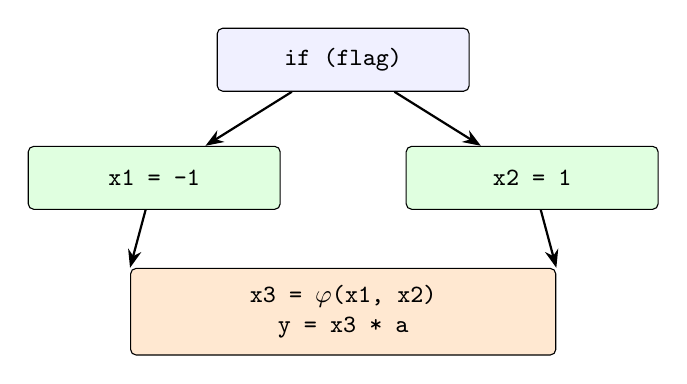
\begin{tikzpicture}[
  every node/.style={font=\small\ttfamily},
  b/.style={draw,rounded corners=2pt,minimum width=3.2cm,minimum height=0.8cm,fill=blue!6},
  e/.style={-{Stealth[length=2.3mm]},thick}]
 \node[b] (t) at (0,0) {if (flag)};
 \node[b,fill=green!12] (l) at (-2.4,-1.5) {x1 = -1};
 \node[b,fill=green!12] (r) at (2.4,-1.5) {x2 = 1};
 \node[b,fill=orange!18,minimum width=5.4cm,minimum height=1.1cm,align=center] (j) at (0,-3.2) {x3 = $\varphi$(x1, x2)\\ y = x3 * a};
 \draw[e] (t) -- (l); \draw[e] (t) -- (r); \draw[e] (l) -- (j.north west); \draw[e] (r) -- (j.north east);
\end{tikzpicture}
\end{center}

%====================================================================
\section{Syntax-Directed Definitions (SDD)}
%====================================================================

\subsection{Why do we need them? Syntax is not enough}
So far, parsing has answered only one question: \emph{``Is this string a legal program, and what is its structure?''} A grammar and its parse tree describe \textbf{syntax}. They say nothing about \textbf{meaning} (\emph{semantics}).

For example, the parse tree of \texttt{3 * 5 + 4} shows that $3*5$ is grouped first, but nowhere does it contain the number 19. The parse tree of \texttt{a = b * c + d} does not contain any machine or three-address instructions either. To translate a program we must \emph{attach extra information to the nodes of the parse tree and compute it}. Typical questions are:
\begin{itemize}[nosep]
\item What is the \textbf{value} of this expression? \hfill (calculators, constant folding)
\item What is the \textbf{type} of this expression? \hfill (type checking)
\item In which temporary or variable is its result \textbf{stored}? \hfill (code generation)
\item Which \textbf{instructions} implement this statement? \hfill (code generation)
\item To which \textbf{label} should control jump if this condition is true? \hfill (control flow)
\end{itemize}
A \textbf{syntax-directed definition} is the formal tool that answers such questions. The idea is simple:
\begin{center}
\fbox{\parbox{0.85\textwidth}{\centering \textbf{Grammar} \;+\; \textbf{extra information (attributes) on every grammar symbol} \;+\; \textbf{small rules (semantic rules) that say how to compute that information from the production being used.}}}
\end{center}
``Syntax-directed'' means that the computation is \emph{driven by the syntactic structure} (the productions) of the input.

\subsection{Attributes}
An \textbf{attribute} is any value that we attach to a grammar symbol. It helps to picture the parse tree as a tree of \emph{records}: every node has the grammar symbol as its name plus a few fields (the attributes). If $X$ is a symbol and $a$ is an attribute, we write $X.a$ for the value of $a$ at a particular node labelled $X$. Attributes can be of any kind: numbers, strings, types, pointers to symbol-table entries, or even whole code sequences.

\begin{center}
\small
\begin{tabular}{@{}l L{6.4cm} l@{}}
\toprule
\textbf{Attribute} & \textbf{Meaning} & \textbf{Typical symbols} \\ \midrule
\at{E}{val} & numeric value of the expression & $E,\,T,\,F$ \\
\at{E}{type} & type of the expression (\texttt{int}, \texttt{float}, \dots) & $E$ \\
\at{\mathbf{id}}{lexeme} & the actual characters of the identifier (supplied by the lexer) & \textbf{id} \\
\at{\mathbf{digit}}{lexval} & numeric value of a digit token (supplied by the lexer) & \textbf{digit}, \textbf{num} \\
\at{E}{addr} & name/temporary holding the result of $E$ & $E$ \\
\at{S}{code} & three-address code for statement $S$ & $S$, $E$, $B$ \\
\at{B}{true}, \at{B}{false} & labels to jump to if $B$ is true or false & $B$ \\
\at{E}{node} & pointer to the syntax-tree node for $E$ & $E$, $T$ \\ \bottomrule
\end{tabular}
\end{center}
Different \emph{occurrences} of the same nonterminal in a production are distinguished by subscripts, e.g., in $E \to E_1 + T$ the $E$ on the left is the \emph{head} and $E_1$ is the $E$ in the body; both have a \textit{val}.

\subsection{Semantic rules: a first tiny example}
A \textbf{semantic rule} is attached to a production and says how to compute one attribute from other attributes \emph{of the symbols in that same production}. For the production $E \to E_1 + T$ the rule
\[
\at{E}{val} = \at{E_1}{val} + \at{T}{val}
\]
says: ``the value of the whole expression is the value of the left sub-expression plus the value of the term.'' Consider the grammar $E \to E + T \mid T,\ T \to \mathbf{digit}$, together with the rules
\begin{center}
\small
\begin{tabular}{@{}l l@{}}
\toprule
\textbf{Production} & \textbf{Semantic rule} \\ \midrule
$E \to E_1 + T$ & $\at{E}{val} = \at{E_1}{val} + \at{T}{val}$ \\
$E \to T$ & $\at{E}{val} = \at{T}{val}$ \\
$T \to \mathbf{digit}$ & $\at{T}{val} = \at{\mathbf{digit}}{lexval}$ \\ \bottomrule
\end{tabular}
\end{center}
Evaluate it on the input \texttt{2 + 3}. The parse tree is $E \Rightarrow E_1 + T$ with $E_1 \Rightarrow T \Rightarrow \mathbf{digit}(2)$ and $T \Rightarrow \mathbf{digit}(3)$. Working \emph{from the leaves upward}:
\begin{enumerate}[nosep]
\item The lexer supplies $\at{\mathbf{digit}}{lexval}=2$ and $3$.
\item $T \to \mathbf{digit}$ gives $\at{T}{val}=2$ (left) and $\at{T}{val}=3$ (right).
\item $E \to T$ gives $\at{E_1}{val}=2$.
\item $E \to E_1 + T$ gives $\at{E}{val}=2+3=5$.
\end{enumerate}
That is all an SDD does: it decorates the parse tree with attribute values by repeatedly applying the rules.

\subsection{Formal definition}
\begin{defbox}{Syntax-Directed Definition (SDD)}
A \textbf{syntax-directed definition} is a context-free grammar together with \textbf{attributes} attached to grammar symbols and \textbf{semantic rules} attached to productions. For a production $A \to \alpha$ every rule has the form
\[
b = f(c_1, c_2, \dots, c_k)
\]
where $f$ is a function and either
\begin{enumerate}[label=(\arabic*),nosep]
\item $b$ is a \textbf{synthesized} attribute of $A$ and $c_1,\dots,c_k$ are attributes of the symbols in $\alpha$ (the children) or of $A$ itself; or
\item $b$ is an \textbf{inherited} attribute of a symbol $B$ in $\alpha$ and $c_1,\dots,c_k$ are attributes of $A$ (the parent) or of symbols in $\alpha$ (the siblings), or of $B$ itself.
\end{enumerate}
\end{defbox}

\subsection{Synthesized and inherited attributes}
\begin{notebox}{Analogy}
Think of the parse tree as a company. A \textbf{synthesized} attribute is a \emph{report sent up} to the manager: the manager's value is built from the reports of the subordinates (e.g., the value of $2+3$ is built from the values of $2$ and $3$). An \textbf{inherited} attribute is an \emph{instruction or information passed down or across}, from a parent or from siblings (e.g., the declared type \texttt{float} is passed down to every identifier in \texttt{float a, b, c}).
\end{notebox}

\begin{itemize}
\item A \textbf{synthesized attribute} at a parse-tree node $N$ is computed from attributes of $N$'s \emph{children} (and $N$ itself). Information flows \emph{bottom-up}. Terminals have synthesized attributes only (supplied by the lexer, e.g., \at{\mathbf{digit}}{lexval}).
\item An \textbf{inherited attribute} at $N$ is computed from attributes of $N$'s \emph{parent and siblings}. Information flows \emph{top-down / sideways}. Useful when the structure of the parse tree does not match the abstract syntax, e.g., passing a type to a list of identifiers, or passing the label to jump to.
\end{itemize}

\begin{examplebox}{Example: synthesized attributes only (desk calculator)}
\begin{center}
\small
\begin{tabular}{@{}l l@{}}
\toprule
\textbf{Production} & \textbf{Semantic rules} \\ \midrule
$L \to E\ \mathbf{n}$ & $\at{L}{val} = \at{E}{val}$ \\
$E \to E_1 + T$ & $\at{E}{val} = \at{E_1}{val} + \at{T}{val}$ \\
$E \to T$ & $\at{E}{val} = \at{T}{val}$ \\
$T \to T_1 * F$ & $\at{T}{val} = \at{T_1}{val} \times \at{F}{val}$ \\
$T \to F$ & $\at{T}{val} = \at{F}{val}$ \\
$F \to (\,E\,)$ & $\at{F}{val} = \at{E}{val}$ \\
$F \to \mathbf{digit}$ & $\at{F}{val} = \at{\mathbf{digit}}{lexval}$ \\ \bottomrule
\end{tabular}
\end{center}

\begin{figure}[H]
\centering
\begin{tikzpicture}[
  every node/.style={font=\small},
  nd/.style={inner sep=1.5pt,align=center}]
 \node[nd] (L) at (0,0) {$L$\\[-1pt]{\scriptsize $val=19$}};
 \node[nd] (E) at (-1.4,-1.5) {$E$\\[-1pt]{\scriptsize $val=19$}};
 \node[nd] (n) at (1.4,-1.5) {\textbf{n}};
 \node[nd] (E1) at (-3.2,-3) {$E$\\[-1pt]{\scriptsize $val=15$}};
 \node[nd] (p) at (-1.4,-3) {$+$};
 \node[nd] (T4) at (0.4,-3) {$T$\\[-1pt]{\scriptsize $val=4$}};
 \node[nd] (T1) at (-3.2,-4.5) {$T$\\[-1pt]{\scriptsize $val=15$}};
 \node[nd] (F4) at (0.4,-4.5) {$F$\\[-1pt]{\scriptsize $val=4$}};
 \node[nd] (T3) at (-4.6,-6) {$T$\\[-1pt]{\scriptsize $val=3$}};
 \node[nd] (st) at (-3.2,-6) {$*$};
 \node[nd] (F5) at (-1.8,-6) {$F$\\[-1pt]{\scriptsize $val=5$}};
 \node[nd] (d4) at (0.4,-6) {\textbf{digit}\\[-1pt]{\scriptsize $lexval=4$}};
 \node[nd] (F3) at (-4.6,-7.5) {$F$\\[-1pt]{\scriptsize $val=3$}};
 \node[nd] (d5) at (-1.8,-7.5) {\textbf{digit}\\[-1pt]{\scriptsize $lexval=5$}};
 \node[nd] (d3) at (-4.6,-9) {\textbf{digit}\\[-1pt]{\scriptsize $lexval=3$}};
 \foreach \a/\b in {L/E,L/n,E/E1,E/p,E/T4,E1/T1,T1/T3,T1/st,T1/F5,T4/F4,F4/d4,T3/F3,F5/d5,F3/d3}
   \draw[gray] (\a.south)--(\b.north);
\end{tikzpicture}
\caption{Annotated parse tree for \texttt{3*5+4 n}. Each node shows the value of its synthesized attribute \textit{val}.}
\end{figure}

\paragraph{How to read the figure (evaluation recipe).}
\begin{enumerate}[nosep]
\item The lexer supplies the \textit{lexval} of every \textbf{digit} leaf (3, 5, 4).
\item Each $F \to \mathbf{digit}$ copies it into \at{F}{val}; each $T \to F$ copies it up again.
\item $T \to T_1 * F$ is applied once both its children are known: $3 \times 5 = 15$.
\item $E \to E_1 + T$ then adds $15 + 4 = 19$, and $L \to E\,\mathbf{n}$ passes $19$ to the root.
\end{enumerate}
Every node is computed \emph{after} its children, i.e., in \textbf{post-order}. This is natural for synthesized attributes, and it is exactly the order in which an LR parser performs reductions.
\end{examplebox}

\subsection{Annotated parse trees and dependency graphs}
An \textbf{annotated parse tree} shows the attribute values at every node. To evaluate attributes we build a \textbf{dependency graph}: one node per attribute instance, and an edge $x \to y$ whenever $y$ is computed from $x$. A valid evaluation order is any \emph{topological order} of this graph; if the graph has a cycle, no order exists.

\begin{figure}[H]
\centering
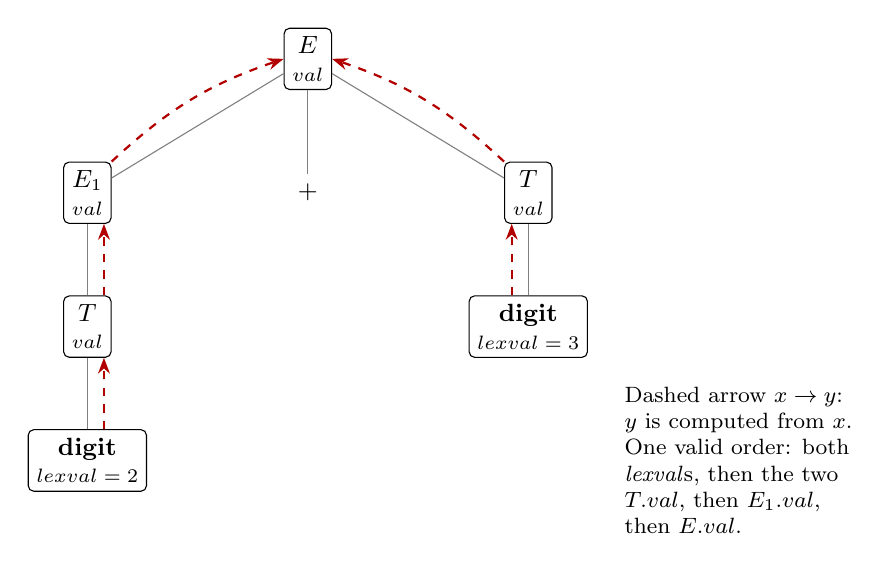
\begin{tikzpicture}[
  every node/.style={font=\small},
  nd/.style={draw,rounded corners=2pt,inner sep=3pt,align=center,fill=white},
  dep/.style={-{Stealth[length=2mm]},dashed,red!70!black,thick}]
 \node[nd] (E)  at (0,0) {$E$\\[-1pt]{\scriptsize $val$}};
 \node[nd] (E1) at (-2.8,-1.7) {$E_1$\\[-1pt]{\scriptsize $val$}};
 \node (pl) at (0,-1.7) {$+$};
 \node[nd] (T)  at (2.8,-1.7) {$T$\\[-1pt]{\scriptsize $val$}};
 \node[nd] (T1) at (-2.8,-3.4) {$T$\\[-1pt]{\scriptsize $val$}};
 \node[nd] (d3) at (2.8,-3.4) {\textbf{digit}\\[-1pt]{\scriptsize $lexval=3$}};
 \node[nd] (d2) at (-2.8,-5.1) {\textbf{digit}\\[-1pt]{\scriptsize $lexval=2$}};
 \foreach \a/\b in {E/E1,E/pl,E/T,E1/T1,T/d3,T1/d2} \draw[gray] (\a)--(\b);
 \draw[dep] ([xshift=6pt]d2.north) -- ([xshift=6pt]T1.south);
 \draw[dep] ([xshift=6pt]T1.north) -- ([xshift=6pt]E1.south);
 \draw[dep] (E1.north east) to[bend left=12] (E.west);
 \draw[dep] ([xshift=-6pt]d3.north) -- ([xshift=-6pt]T.south);
 \draw[dep] (T.north west) to[bend right=12] (E.east);
 \node[font=\footnotesize,align=left,anchor=west] at (3.9,-5.1) {Dashed arrow $x\to y$:\\ $y$ is computed from $x$.\\ One valid order: both\\ \textit{lexval}s, then the two\\ $T.val$, then $E_1.val$,\\ then $E.val$.};
\end{tikzpicture}
\caption{Dependency graph for \texttt{2 + 3} under the SDD of this section (every attribute is synthesized, so every arrow points \emph{up}).}
\end{figure}

\begin{notebox}{A circular definition}
For $A \to B$ with the rules $\at{A}{s} = \at{B}{i} + 1$ and $\at{B}{i} = \at{A}{s} \times 2$, the value of \at{A}{s} needs \at{B}{i}, which needs \at{A}{s}. The dependency graph has a \emph{cycle}, so no evaluation order exists. A good SDD must be \emph{non-circular}; the classes S-attributed and L-attributed below guarantee this automatically.
\end{notebox}

\begin{notebox}{Side effects}
A semantic rule may also do something besides computing a value, e.g., \textit{addType}$(\mathit{entry},\,t)$ writes into the symbol table, \textit{print} writes to the output, and \textit{gen} emits an instruction. Such rules are called \textbf{side effects}; they are fine as long as the order in which they run does not change the result (or the order is controlled, which is the job of an SDT).
\end{notebox}

\begin{examplebox}{Example: inherited attributes (declaration list)}
\begin{center}
\small
\begin{tabular}{@{}l l@{}}
\toprule
\textbf{Production} & \textbf{Semantic rules} \\ \midrule
$D \to T\ L$ & $\at{L}{inh} = \at{T}{type}$ \\
$T \to \mathbf{int}$ & $\at{T}{type} = integer$ \\
$T \to \mathbf{float}$ & $\at{T}{type} = float$ \\
$L \to L_1\,,\ \mathbf{id}$ & $\at{L_1}{inh} = \at{L}{inh}$;\ \ $\mathit{addType}(\at{\mathbf{id}}{entry},\ \at{L}{inh})$ \\
$L \to \mathbf{id}$ & $\mathit{addType}(\at{\mathbf{id}}{entry},\ \at{L}{inh})$ \\ \bottomrule
\end{tabular}
\end{center}

For the input \texttt{float id$_1$, id$_2$} the dashed arrows in Fig.~\ref{fig:inh} are the dependency-graph edges. The type is passed \emph{down and across} from $T$ to $L$, then down through the list to each identifier.

\begin{figure}[H]
\centering
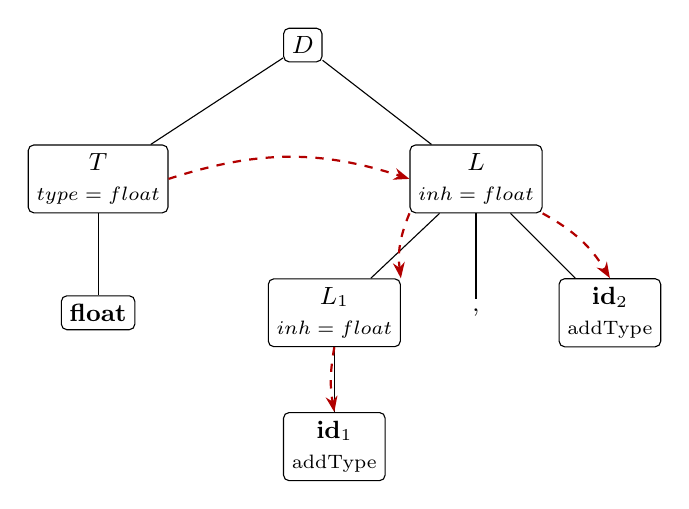
\begin{tikzpicture}[
  every node/.style={font=\small},
  nd/.style={draw,rounded corners=2pt,inner sep=3pt,align=center,fill=white},
  dep/.style={-{Stealth[length=2mm]},dashed,red!70!black,thick}]
 \node[nd] (D)  at (0,0) {$D$};
 \node[nd] (T)  at (-2.6,-1.7) {$T$\\{\scriptsize $type=float$}};
 \node[nd] (L)  at (2.2,-1.7) {$L$\\{\scriptsize $inh=float$}};
 \node[nd] (fl) at (-2.6,-3.4) {\textbf{float}};
 \node[nd] (L1) at (0.4,-3.4) {$L_1$\\{\scriptsize $inh=float$}};
 \node (cm) at (2.2,-3.4) {$,$};
 \node[nd] (i2) at (3.9,-3.4) {\textbf{id}$_2$\\{\scriptsize addType}};
 \node[nd] (i1) at (0.4,-5.1) {\textbf{id}$_1$\\{\scriptsize addType}};
 \foreach \a/\b in {D/T,D/L,T/fl,L/L1,L/cm,L/i2,L1/i1} \draw (\a)--(\b);
 \draw[dep] (T.east) to[bend left=18] (L.west);
 \draw[dep] (L.south west) to[bend right=15] (L1.north east);
 \draw[dep] (L.south east) to[bend left=15] (i2.north);
 \draw[dep] (L1.south) to[bend right=10] (i1.north);
\end{tikzpicture}
\caption{Parse tree for \texttt{float id$_1$, id$_2$} with dependency edges (dashed) for the inherited attribute \textit{inh}.}
\label{fig:inh}
\end{figure}

\textbf{One valid evaluation order} (any topological order of the dependency graph works):
\begin{enumerate}[nosep,label=(\arabic*)]
\item $T.\mathit{type}=\mathit{float}$ \hfill ($T\to\mathbf{float}$; depends on nothing)
\item $L.\mathit{inh}=T.\mathit{type}$ \hfill ($D\to T\,L$)
\item $L_1.\mathit{inh}=L.\mathit{inh}$ \hfill ($L\to L_1\,,\,\mathbf{id}_2$)
\item $\mathit{addType}(\mathbf{id}_2.\mathit{entry},\ L.\mathit{inh})$ \hfill (the identifier after the comma)
\item $\mathit{addType}(\mathbf{id}_1.\mathit{entry},\ L_1.\mathit{inh})$ \hfill ($L_1\to\mathbf{id}_1$)
\end{enumerate}
Steps (4) and (5) do not depend on each other, so they may be swapped; both identifiers end up with type \textit{float} either way.
\end{examplebox}

\subsection{Classes of SDDs that are easy to implement}

\begin{defbox}{S-attributed and L-attributed definitions}
\begin{itemize}
\item An SDD is \textbf{S-attributed} if \emph{every attribute is synthesized}. It can be evaluated in any bottom-up order, e.g., during LR parsing, at the time of reduction.
\item An SDD is \textbf{L-attributed} if each attribute is either synthesized, or inherited such that, for a production $A \to X_1 X_2 \cdots X_n$, the inherited attribute of $X_i$ depends only on:
 \begin{enumerate}[label=(\alph*),nosep]
 \item inherited attributes of $A$, and
 \item attributes (inherited or synthesized) of $X_1,\dots,X_{i-1}$ (the symbols to its \emph{left}), and
 \item attributes of $X_i$ itself, provided there is no cycle.
 \end{enumerate}
 Evaluation is possible in a single left-to-right depth-first traversal (e.g., during top-down/LL parsing).
\end{itemize}
Every S-attributed SDD is also L-attributed.
\end{defbox}

\begin{examplebox}{Not L-attributed}
For $A \to B\,C$, the rule $\at{C}{i} = \at{B}{s}$ is fine (the inherited attribute of $C$ uses its \emph{left} sibling $B$). But the rule $\at{B}{i} = f(\at{C}{x})$ makes the inherited attribute of $B$ depend on its \emph{right} sibling $C$, so the SDD is \emph{not} L-attributed.
\end{examplebox}

\begin{figure}[H]
\centering
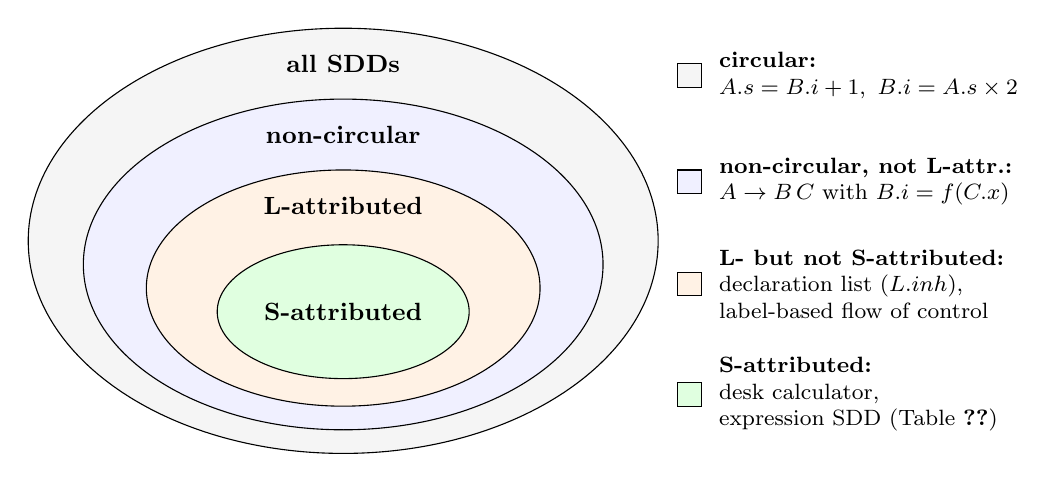
\begin{tikzpicture}[lab/.style={font=\small\bfseries,align=center},
  ex/.style={font=\footnotesize,align=left,anchor=west}]
 \draw[fill=gray!8]    (0,0)    ellipse (4.0cm and 2.7cm);
 \draw[fill=blue!6]    (0,-0.3) ellipse (3.3cm and 2.1cm);
 \draw[fill=orange!10] (0,-0.6) ellipse (2.5cm and 1.5cm);
 \draw[fill=green!12]  (0,-0.9) ellipse (1.6cm and 0.85cm);
 \node[lab] at (0,2.25) {all SDDs};
 \node[lab] at (0,1.35) {non-circular};
 \node[lab] at (0,0.45) {L-attributed};
 \node[lab] at (0,-0.9) {S-attributed};
 \node[draw,fill=gray!8,minimum size=3mm,inner sep=0pt] at (4.4,2.1) {};
 \node[ex] at (4.65,2.1) {\textbf{circular:}\\ $A.s=B.i+1,\ B.i=A.s\times 2$};
 \node[draw,fill=blue!6,minimum size=3mm,inner sep=0pt] at (4.4,0.75) {};
 \node[ex] at (4.65,0.75) {\textbf{non-circular, not L-attr.:}\\ $A\to B\,C$ with $B.i=f(C.x)$};
 \node[draw,fill=orange!10,minimum size=3mm,inner sep=0pt] at (4.4,-0.55) {};
 \node[ex] at (4.65,-0.55) {\textbf{L- but not S-attributed:}\\ declaration list ($L.inh$),\\ label-based flow of control};
 \node[draw,fill=green!12,minimum size=3mm,inner sep=0pt] at (4.4,-1.95) {};
 \node[ex] at (4.65,-1.95) {\textbf{S-attributed:}\\ desk calculator,\\ expression SDD (Table~\ref{tab:expr-sdd})};
\end{tikzpicture}
\caption{How the classes of SDDs nest, with an example of each.}
\end{figure}

\subsection{SDD for constructing syntax trees}
\label{sec:sddtree}
Syntax trees can be built using synthesized attribute \textit{node}, which points to the root of a (sub)tree, and constructor functions $\mathit{Node}(op, c_1,\dots)$ and $\mathit{Leaf}(\mathbf{id}, entry)$ / $\mathit{Leaf}(\mathbf{num}, val)$.

\begin{center}
\small
\begin{tabular}{@{}l l@{}}
\toprule
\textbf{Production} & \textbf{Semantic rules} \\ \midrule
$E \to E_1 + T$ & $\at{E}{node} = \mathbf{new}\ \mathit{Node}(\tok{'+'},\ \at{E_1}{node},\ \at{T}{node})$ \\
$E \to E_1 - T$ & $\at{E}{node} = \mathbf{new}\ \mathit{Node}(\tok{'-'},\ \at{E_1}{node},\ \at{T}{node})$ \\
$E \to T$ & $\at{E}{node} = \at{T}{node}$ \\
$T \to (\,E\,)$ & $\at{T}{node} = \at{E}{node}$ \\
$T \to \mathbf{id}$ & $\at{T}{node} = \mathbf{new}\ \mathit{Leaf}(\mathbf{id},\ \at{\mathbf{id}}{entry})$ \\
$T \to \mathbf{num}$ & $\at{T}{node} = \mathbf{new}\ \mathit{Leaf}(\mathbf{num},\ \at{\mathbf{num}}{val})$ \\ \bottomrule
\end{tabular}
\end{center}
\textbf{Building a DAG directly.} If each $\mathbf{new}\ \mathit{Node}(\dots)$ / $\mathbf{new}\ \mathit{Leaf}(\dots)$ is replaced by the find-or-create routine of Section~\ref{sec:vn} (which returns an existing node when an identical one exists), the same SDD builds a DAG during parsing, and $\at{E}{node}$ holds a value number.

This is S-attributed. If the grammar is made LL by eliminating left recursion, the same tree is built with an inherited attribute (see the L-attributed SDT in Section~\ref{sec:lattr}).

%====================================================================
\section{Syntax-Directed Translation Schemes (SDT)}
%====================================================================

\subsection{From specification to implementation}
An SDD tells us \emph{what} every attribute must equal, but it does not say \emph{when} each rule should run. A real compiler, however, runs the rules \emph{while it is parsing}, in one definite order, and often without ever building the whole parse tree. A \textbf{syntax-directed translation scheme (SDT)} solves this: it takes the program fragments of the rules and writes them \emph{inside the production body, at the exact position where they should run}.

The same rule written both ways:
\begin{center}
\small
\begin{tabular}{@{}l l@{}}
\toprule
\textbf{SDD} (specification) & \textbf{SDT} (implementation) \\ \midrule
\begin{tabular}[t]{@{}l@{}}$E \to E_1 + T$\\ \ \ rule: $\at{E}{val} = \at{E_1}{val} + \at{T}{val}$\end{tabular}
&
$E \to E_1 + T\ \ \{\ \at{E}{val} = \at{E_1}{val} + \at{T}{val}\ \}$ \\ \bottomrule
\end{tabular}
\end{center}

\begin{center}
\small
\begin{tabular}{@{}L{3.2cm} L{5.6cm} L{5.6cm}@{}}
\toprule
 & \textbf{SDD} & \textbf{SDT} \\ \midrule
Nature & High-level specification: rules attached to productions & Concrete implementation: actions embedded in productions \\
Order of evaluation & Not specified (any order consistent with dependencies) & Explicit: actions run in the left-to-right order of the production body \\
Rules/actions & Written next to the production & Written in braces $\{\dots\}$ inside the body \\
Used for & Designing and reasoning about the translation & Building the actual translator \\ \bottomrule
\end{tabular}
\end{center}

\subsection{Definition and the meaning of an action's position}
\begin{defbox}{Syntax-Directed Translation Scheme}
A \textbf{syntax-directed translation scheme} (SDT) is a context-free grammar with \textbf{program fragments} (\emph{semantic actions}) embedded within the production bodies, written in braces. The position of an action defines \emph{when} it is executed during parsing.
\[
B \to X\ \{a\}\ Y
\]
Here action $a$ is executed after $X$ has been recognised (and before $Y$).
\end{defbox}

\paragraph{How an SDT is executed.} Imagine the parse tree in which every action appears as an \emph{extra child}, exactly at the position where it is written in the production. Perform a \textbf{depth-first traversal from left to right}; whenever the traversal reaches an action, it is executed. Figure~\ref{fig:actiontree} shows this for a scheme that translates infix to postfix: \texttt{expr $\to$ expr + term \{print('+')\}\ |\ expr - term \{print('-')\}\ |\ term} and \texttt{term $\to$ digit \{print(digit)\}}.

\begin{figure}[htbp]
\centering
\resizebox{0.95\textwidth}{!}{%
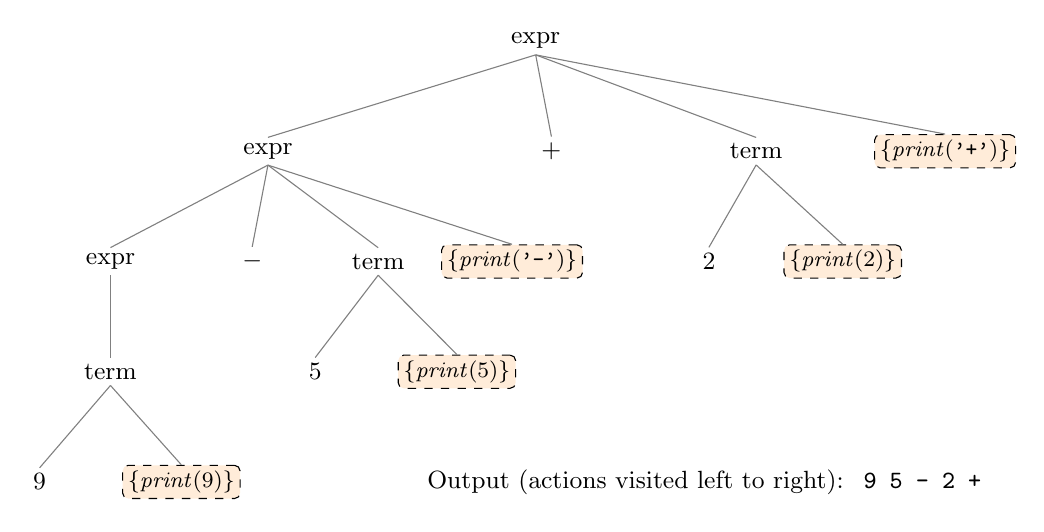
\begin{tikzpicture}[
  every node/.style={font=\small},
  nd/.style={inner sep=2pt},
  act/.style={inner sep=2pt,draw,dashed,rounded corners=2pt,fill=orange!15,font=\footnotesize}]
 \node[nd] (e0) at (0,0) {expr};
 \node[nd] (e1) at (-3.4,-1.4) {expr};
 \node[nd] (p1) at (0.2,-1.4) {$+$};
 \node[nd] (t2) at (2.8,-1.4) {term};
 \node[act] (a2) at (5.2,-1.4) {$\{\mathit{print}(\texttt{'+'})\}$};
 \node[nd] (e2) at (-5.4,-2.8) {expr};
 \node[nd] (m1) at (-3.6,-2.8) {$-$};
 \node[nd] (t5) at (-2.0,-2.8) {term};
 \node[act] (am) at (-0.3,-2.8) {$\{\mathit{print}(\texttt{'-'})\}$};
 \node[nd] (d2) at (2.2,-2.8) {2};
 \node[act] (ad2) at (3.9,-2.8) {$\{\mathit{print}(2)\}$};
 \node[nd] (t9) at (-5.4,-4.2) {term};
 \node[nd] (d5) at (-2.8,-4.2) {5};
 \node[act] (ad5) at (-1.0,-4.2) {$\{\mathit{print}(5)\}$};
 \node[nd] (d9) at (-6.3,-5.6) {9};
 \node[act] (ad9) at (-4.5,-5.6) {$\{\mathit{print}(9)\}$};
 \foreach \a/\b in {e0/e1,e0/p1,e0/t2,e0/a2,e1/e2,e1/m1,e1/t5,e1/am,e2/t9,t5/d5,t5/ad5,t2/d2,t2/ad2,t9/d9,t9/ad9}
   \draw[gray] (\a.south)--(\b.north);
 \node[anchor=west] at (-1.5,-5.6) {Output (actions visited left to right): \ \texttt{9\ 5\ -\ 2\ +}};
\end{tikzpicture}}
\caption{Parse tree of \texttt{9-5+2} with actions (dashed boxes) as extra children. Visiting the tree depth-first, left to right, executes the actions in the order $9,\,5,\,-,\,2,\,+$, producing the postfix form.}
\label{fig:actiontree}
\end{figure}

In practice the parser does not need to build this tree. A top-down parser executes an action at the corresponding point of its recursive-descent procedure. A bottom-up (LR) parser can only act when it \emph{reduces}: an action at the right end of a body runs at that reduction (a postfix SDT, next subsection), while an action in the middle of a body needs a marker nonterminal (Section~\ref{sec:marker}).

\subsection{Postfix translation schemes}
If the grammar is LR-parsable and the SDD is \textbf{S-attributed}, we can build an SDT with every action at the \emph{right end} of its production (a \textbf{postfix SDT}). The actions then execute at \emph{reduction time}, so the attribute of each grammar symbol can be stored beside it on the parser stack.

\begin{examplebox}{Postfix SDT for the desk calculator}
\begin{align*}
L &\to E\ \mathbf{n} &&\{\ \mathit{print}(\at{E}{val})\ \}\\
E &\to E_1 + T &&\{\ \at{E}{val} = \at{E_1}{val} + \at{T}{val}\ \}\\
E &\to T &&\{\ \at{E}{val} = \at{T}{val}\ \}\\
T &\to T_1 * F &&\{\ \at{T}{val} = \at{T_1}{val} \times \at{F}{val}\ \}\\
T &\to F &&\{\ \at{T}{val} = \at{F}{val}\ \}\\
F &\to (\,E\,) &&\{\ \at{F}{val} = \at{E}{val}\ \}\\
F &\to \mathbf{digit} &&\{\ \at{F}{val} = \at{\mathbf{digit}}{lexval}\ \}
\end{align*}
\end{examplebox}

\paragraph{Implementation on the LR parse stack.} Each stack entry holds a grammar symbol and its attribute value. When $A \to X Y Z$ is reduced, the actions read the values in the top three entries (\texttt{stack[top-2].val}, \texttt{stack[top-1].val}, \texttt{stack[top].val}), compute \at{A}{val}, pop three entries, and push $A$ with the new value.

\begin{center}
\small
\begin{tabular}{@{}l l l l@{}}
\toprule
\textbf{Stack (symbol:val)} & \textbf{Remaining input} & \textbf{Action} \\ \midrule
$\$$ & \texttt{3 * 5 + 4 n} & shift \\
$\$\ \mathbf{digit}{:}3$ & \texttt{* 5 + 4 n} & reduce $F\to\mathbf{digit}$ \\
$\$\ F{:}3$ & \texttt{* 5 + 4 n} & reduce $T\to F$ \\
$\$\ T{:}3$ & \texttt{* 5 + 4 n} & shift $*$, shift \textbf{digit} \\
$\$\ T{:}3\ *\ \mathbf{digit}{:}5$ & \texttt{+ 4 n} & reduce $F\to\mathbf{digit}$ \\
$\$\ T{:}3\ *\ F{:}5$ & \texttt{+ 4 n} & reduce $T\to T*F$ \quad ($3\times5=15$) \\
$\$\ T{:}15$ & \texttt{+ 4 n} & reduce $E\to T$ \\
$\$\ E{:}15$ & \texttt{+ 4 n} & shift $+$, shift \textbf{digit}, reduce to $T{:}4$ \\
$\$\ E{:}15\ +\ T{:}4$ & \texttt{n} & reduce $E\to E+T$ \quad ($15+4=19$) \\
$\$\ E{:}19$ & \texttt{n} & shift \textbf{n}, reduce $L\to E\,\mathbf{n}$, print 19 \\ \bottomrule
\end{tabular}
\end{center}

\subsection{SDTs with actions inside productions}
When an action is in the middle of a production, it is performed \emph{immediately after all grammar symbols to its left have been matched}. A top-down parser does exactly that: the action is just a statement placed at that point of the recursive-descent procedure. An LR parser cannot: it only takes decisions at reductions, so a mid-production action must first be turned into a reduction using a marker nonterminal (Section~\ref{sec:marker}).

\begin{center}
\small
\begin{tabular}{@{}L{3.6cm} L{5.4cm} L{5.4cm}@{}}
\toprule
\textbf{Where the action is} & \textbf{Top-down (LL / recursive descent)} & \textbf{Bottom-up (LR)} \\ \midrule
At the right end & run after the last symbol of the body is matched & run at the reduction of the body \\
In the middle & run at that point of the procedure & not possible directly: introduce a marker $M\to\varepsilon$ \\ \bottomrule
\end{tabular}
\end{center}

\begin{examplebox}{Example: infix to postfix (action placed after the operand)}
\begin{align*}
E &\to T\ R\\
R &\to +\ T\ \{\ \mathit{print}(\tok{'+'})\ \}\ R_1 \mid -\ T\ \{\ \mathit{print}(\tok{'-'})\ \}\ R_1 \mid \varepsilon\\
T &\to \mathbf{num}\ \{\ \mathit{print}(\at{\mathbf{num}}{val})\ \}
\end{align*}
For \texttt{9-5+2} the output is \texttt{95-2+}.
\end{examplebox}

\subsection{Marker nonterminals (actions in the middle, for bottom-up parsing)}
\label{sec:marker}
Suppose an action must appear in the middle of a production, e.g., $B \to X\ \{a\}\ Y$. For an LR parser we replace the action by a \textbf{marker nonterminal} $M$ with an empty production:
\[
B \to X\ M\ Y, \qquad M \to \varepsilon\ \{a\}
\]
The action $a$ is then executed upon reducing $M \to \varepsilon$, which happens exactly when $X$ is on top of the stack and $Y$ has not been read yet.

\begin{examplebox}{Example: the infix-to-postfix scheme under LR parsing}
The top-down scheme $R \to +\ T\ \{\mathit{print}(\tok{'+'})\}\ R_1$ has its action in the middle. For an LR parser we write
\[
R \to +\ T\ M\ R_1, \qquad M \to \varepsilon\ \{\ \mathit{print}(\tok{'+'})\ \}
\]
When $M\to\varepsilon$ is reduced, the operand $T$ has just been reduced (and printed), so the output order is unchanged: $9\,5\,-\,2\,+$ for \texttt{9-5+2}.
\end{examplebox}

\begin{pitfallbox}{Markers can create conflicts}
A marker forces the parser to decide to reduce $M\to\varepsilon$ \emph{before} it knows which production will finally be used. If two productions start with the same symbols, say $S\to X\,M\,Y \mid X\,Z$, the parser must choose, using only the next input token, whether to reduce $M$. If $Y$ and $Z$ can start with the same token, the result is a conflict and the grammar is no longer LR(1). The markers in backpatching ($M$ before a statement, $N$ before \textbf{else}) are safe because they always occur at a point where the parser can already tell what is coming.
\end{pitfallbox}

We will use markers $M$ and $N$ extensively in backpatching (Section~\ref{sec:backpatch}).

\subsection{Eliminating left recursion from an SDT}
\label{sec:leftrec}
A top-down parser cannot use a left-recursive grammar such as $E\to E_1+T$, but the \emph{translation} we want (a left-associative tree or value) is naturally defined by that grammar. The fix is to rewrite the grammar \emph{and} the actions together, using an inherited attribute that carries the result built so far.

\begin{defbox}{General transformation}
\begin{align*}
A &\to A_1\,Y\ \{\ \at{A}{a}=g(\at{A_1}{a},\ \at{Y}{y})\ \}\ \mid\ X\ \{\ \at{A}{a}=f(\at{X}{x})\ \}
\intertext{becomes}
A &\to X\ \{\ \at{R}{i}=f(\at{X}{x})\ \}\ R\ \{\ \at{A}{a}=\at{R}{s}\ \}\\
R &\to Y\ \{\ \at{R_1}{i}=g(\at{R}{i},\ \at{Y}{y})\ \}\ R_1\ \{\ \at{R}{s}=\at{R_1}{s}\ \}\ \mid\ \varepsilon\ \{\ \at{R}{s}=\at{R}{i}\ \}
\end{align*}
$R.i$ (inherited) carries the value accumulated \emph{so far}; $R.s$ (synthesized) carries the final result back to the top.
\end{defbox}

\begin{examplebox}{Example: evaluating $9-5+2$ with a left-recursion-free grammar}
The left-recursive grammar $E\to E_1+T\mid E_1-T\mid T$, $T\to\mathbf{num}$, with $E.val=E_1.val\pm T.val$, becomes
\begin{align*}
E &\to T\ \{\ R.i=T.val\ \}\ R\ \{\ E.val=R.s\ \}\\
R &\to +\ T\ \{\ R_1.i=R.i+T.val\ \}\ R_1\ \{\ R.s=R_1.s\ \}\\
  &\mid\ -\ T\ \{\ R_1.i=R.i-T.val\ \}\ R_1\ \{\ R.s=R_1.s\ \}\ \mid\ \varepsilon\ \{\ R.s=R.i\ \}\\
T &\to \mathbf{num}\ \{\ T.val=\mathbf{num}.lexval\ \}
\end{align*}

\begin{figure}[H]
\centering
\resizebox{0.95\textwidth}{!}{%
\begin{tikzpicture}[
  every node/.style={font=\small},
  nd/.style={inner sep=1.5pt,align=center}]
 \node[nd] (E)  at (0,0) {$E$\\[-1pt]{\scriptsize $val=6$}};
 \node[nd] (T0) at (-2.6,-1.6) {$T$\\[-1pt]{\scriptsize $val=9$}};
 \node[nd] (R0) at (1.4,-1.6) {$R$\\[-1pt]{\scriptsize $i=9,\ s=6$}};
 \node[nd] (n9) at (-2.6,-3.2) {\textbf{num}\\[-1pt]{\scriptsize $9$}};
 \node[nd] (m1) at (-0.4,-3.2) {$-$};
 \node[nd] (T5) at (1.2,-3.2) {$T$\\[-1pt]{\scriptsize $val=5$}};
 \node[nd] (R1) at (3.8,-3.2) {$R$\\[-1pt]{\scriptsize $i=4,\ s=6$}};
 \node[nd] (n5) at (1.2,-4.8) {\textbf{num}\\[-1pt]{\scriptsize $5$}};
 \node[nd] (p1) at (2.4,-4.8) {$+$};
 \node[nd] (T2) at (4.0,-4.8) {$T$\\[-1pt]{\scriptsize $val=2$}};
 \node[nd] (R2) at (6.2,-4.8) {$R$\\[-1pt]{\scriptsize $i=6,\ s=6$}};
 \node[nd] (n2) at (4.0,-6.4) {\textbf{num}\\[-1pt]{\scriptsize $2$}};
 \node[nd] (ep) at (6.2,-6.4) {$\varepsilon$};
 \foreach \a/\b in {E/T0,E/R0,T0/n9,R0/m1,R0/T5,R0/R1,T5/n5,R1/p1,R1/T2,R1/R2,T2/n2,R2/ep}
   \draw[gray] (\a.south)--(\b.north);
\end{tikzpicture}}
\caption{Annotated parse tree for \texttt{9-5+2}. The inherited $R.i$ flows down and to the right ($9\to4\to6$: first $9-5$, then $4+2$); the synthesized $R.s$ then carries the final $6$ back up to $E.val$.}
\end{figure}

The tree leans to the right, but the arithmetic is still left-associative: $(9-5)+2=6$, not $9-(5+2)=2$.
\end{examplebox}

\subsection{Converting an L-attributed SDD into an SDT}
\label{sec:lattr}
\begin{defbox}{Rules for converting an L-attributed SDD to an SDT}
\begin{enumerate}[nosep]
\item \textbf{Inherited attribute} of a nonterminal $X$ in the body: embed the action that computes it \emph{immediately before} $X$ in the body. If several inherited attributes of $X$ depend on one another, order the actions appropriately.
\item \textbf{Synthesized attribute} of the head $A$: place the action that computes it at the \emph{end} of the production body.
\end{enumerate}
\end{defbox}

\begin{examplebox}{Example: syntax tree for a left-recursion-free grammar}
After removing left recursion from $E \to E_1 + T \mid E_1 - T \mid T$:
\begin{align*}
E &\to T\ \{\ \at{R}{i} = \at{T}{node}\ \}\ R\ \{\ \at{E}{node} = \at{R}{s}\ \}\\
R &\to +\ T\ \{\ \at{R_1}{i} = \mathbf{new}\ \mathit{Node}(\tok{'+'},\at{R}{i},\at{T}{node})\ \}\ R_1\ \{\ \at{R}{s} = \at{R_1}{s}\ \}\\
R &\to -\ T\ \{\ \at{R_1}{i} = \mathbf{new}\ \mathit{Node}(\tok{'-'},\at{R}{i},\at{T}{node})\ \}\ R_1\ \{\ \at{R}{s} = \at{R_1}{s}\ \}\\
R &\to \varepsilon\ \{\ \at{R}{s} = \at{R}{i}\ \}\\
T &\to \mathbf{id}\ \{\ \at{T}{node} = \mathbf{new}\ \mathit{Leaf}(\mathbf{id},\at{\mathbf{id}}{entry})\ \}\\
T &\to \mathbf{num}\ \{\ \at{T}{node} = \mathbf{new}\ \mathit{Leaf}(\mathbf{num},\at{\mathbf{num}}{val})\ \}
\end{align*}
Here $R.i$ (inherited) carries the tree built \emph{so far}; $R.s$ (synthesized) returns the final tree. For \texttt{a - 4 + c} the tree $((a - 4) + c)$ is produced with the correct left-associativity.
\end{examplebox}

%====================================================================
\section{Translation of Expressions and Assignments}
%====================================================================

\subsection{SDD for three-address code}
\label{sec:exprtac}
We use the following:
\begin{itemize}
\item \at{E}{addr}: the address (name, constant, or temporary) that holds the value of $E$.
\item \at{E}{code} (or \at{S}{code}): the three-address instructions that evaluate $E$ (or execute $S$).
\item $\mathit{newTemp}()$ (written \textbf{new} \textit{Temp}): returns a fresh temporary $t_1, t_2,\dots$ in successive calls.
\item $\gen{\cdots}$: builds a three-address instruction. $\cc$ denotes concatenation of instruction sequences.
\end{itemize}

\begin{table}[htbp]
\centering
\small
\begin{tabular}{@{}L{3.3cm} L{11.4cm}@{}}
\toprule
\textbf{Production} & \textbf{Semantic rules} \\ \midrule
$S \to \mathbf{id} = E\ ;$ &
$\at{S}{code} = \at{E}{code} \cc \gen{\mathit{top}.\mathit{get}(\at{\mathbf{id}}{lexeme})\ \tok{=}\ \at{E}{addr}}$ \\
$E \to E_1 + E_2$ &
$\at{E}{addr} = \mathbf{new}\ \mathit{Temp}()$\\ &
$\at{E}{code} = \at{E_1}{code} \cc \at{E_2}{code} \cc \gen{\at{E}{addr}\ \tok{=}\ \at{E_1}{addr}\ \tok{+}\ \at{E_2}{addr}}$ \\
$E \to E_1 * E_2$ &
$\at{E}{addr} = \mathbf{new}\ \mathit{Temp}()$\\ &
$\at{E}{code} = \at{E_1}{code} \cc \at{E_2}{code} \cc \gen{\at{E}{addr}\ \tok{=}\ \at{E_1}{addr}\ \tok{*}\ \at{E_2}{addr}}$ \\
$E \to -\,E_1$ &
$\at{E}{addr} = \mathbf{new}\ \mathit{Temp}()$\\ &
$\at{E}{code} = \at{E_1}{code} \cc \gen{\at{E}{addr}\ \tok{=}\ \tok{minus}\ \at{E_1}{addr}}$ \\
$E \to (\,E_1\,)$ &
$\at{E}{addr} = \at{E_1}{addr}$;\quad $\at{E}{code} = \at{E_1}{code}$ \\
$E \to \mathbf{id}$ &
$\at{E}{addr} = \mathit{top}.\mathit{get}(\at{\mathbf{id}}{lexeme})$;\quad $\at{E}{code} = \tok{''}$ \\ \bottomrule
\end{tabular}
\caption{SDD to produce three-address code for expressions and assignments (Dragon Book Fig.~6.19).}
\label{tab:expr-sdd}
\end{table}

\begin{notebox}{Remark}
Here $\mathit{top}$ is the current symbol table; $\mathit{top}.\mathit{get}(\textit{name})$ returns the symbol-table entry. The code of a node is the \emph{concatenation} of its children's code followed by one new instruction, so the instructions are produced in postfix (evaluation) order. The $\at{}{code}$ attribute is a long string, so this SDD is inefficient in practice, which motivates the incremental approach below.
\end{notebox}

The grammar $E\to E_1+E_2\mid E_1*E_2\mid-E_1\mid(E_1)\mid\mathbf{id}$ is ambiguous. Precedence ($-$ highest, then $*$, then $+$) and left-associativity are supplied either by parser-generator declarations or by rewriting the grammar with levels $E, T, F$. This does not change the semantic rules: they are written once per \emph{operator}, whatever the grammar levels are called. The $*$ rule is the $+$ rule with the operator replaced; the rule for binary $-$ and for $/$ is identical again.

\begin{examplebox}{Worked example: $a = b * -c + b * -c\ ;$}
\begin{center}
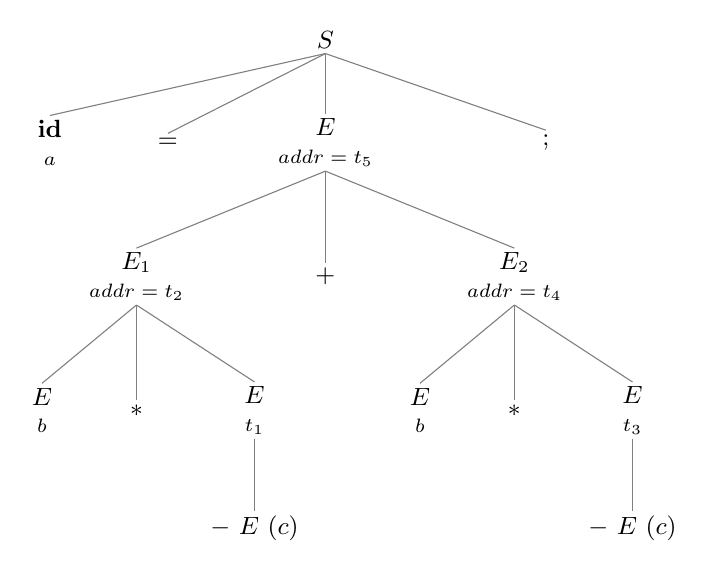
\begin{tikzpicture}[
  every node/.style={font=\small},
  nd/.style={inner sep=1.5pt,align=center}]
 \node[nd] (S)  at (0,0) {$S$};
 \node[nd] (id) at (-3.5,-1.3) {\textbf{id}\\[-1pt]{\scriptsize $a$}};
 \node[nd] (eq) at (-2,-1.3) {$=$};
 \node[nd] (E)  at (0,-1.3) {$E$\\[-1pt]{\scriptsize $addr=t_5$}};
 \node[nd] (sc) at (2.8,-1.3) {$;$};
 \node[nd] (E1) at (-2.4,-3) {$E_1$\\[-1pt]{\scriptsize $addr=t_2$}};
 \node[nd] (pl) at (0,-3) {$+$};
 \node[nd] (E2) at (2.4,-3) {$E_2$\\[-1pt]{\scriptsize $addr=t_4$}};
 \node[nd] (b1) at (-3.6,-4.7) {$E$\\[-1pt]{\scriptsize $b$}};
 \node[nd] (st1) at (-2.4,-4.7) {$*$};
 \node[nd] (m1) at (-0.9,-4.7) {$E$\\[-1pt]{\scriptsize $t_1$}};
 \node[nd] (b2) at (1.2,-4.7) {$E$\\[-1pt]{\scriptsize $b$}};
 \node[nd] (st2) at (2.4,-4.7) {$*$};
 \node[nd] (m2) at (3.9,-4.7) {$E$\\[-1pt]{\scriptsize $t_3$}};
 \node[nd] (c1) at (-0.9,-6.2) {$-\ E\ (c)$};
 \node[nd] (c2) at (3.9,-6.2) {$-\ E\ (c)$};
 \foreach \a/\b in {S/id,S/eq,S/E,S/sc,E/E1,E/pl,E/E2,E1/b1,E1/st1,E1/m1,E2/b2,E2/st2,E2/m2,m1/c1,m2/c2}
   \draw[gray] (\a.south)--(\b.north);
\end{tikzpicture}
\end{center}
Concatenating the code in the order of evaluation gives:
\begin{lstlisting}
t1 = minus c
t2 = b * t1
t3 = minus c
t4 = b * t3
t5 = t2 + t4
a  = t5
\end{lstlisting}
\end{examplebox}

\subsection{Incremental translation (SDT with \texttt{gen} emitting directly)}
Building \at{E}{code} as a string copies code repeatedly. In an \emph{incremental} scheme, $\mathit{gen}()$ \textbf{appends} the instruction to an output stream/array as soon as the action is executed. The code attribute is not stored. Since actions run in the correct order (postfix), the instructions come out in the right order.

\begin{table}[htbp]
\centering
\small
\begin{tabular}{@{}L{2.6cm} L{12cm}@{}}
\toprule
\textbf{Production} & \textbf{Translation scheme (actions in braces)} \\ \midrule
$S \to \mathbf{id} = E\ ;$ & $\{\ \mathit{gen}(\mathit{top}.\mathit{get}(\at{\mathbf{id}}{lexeme})\ \tok{=}\ \at{E}{addr});\ \}$ \\
$E \to E_1 + E_2$ & $\{\ \at{E}{addr} = \mathbf{new}\ \mathit{Temp}();\ \mathit{gen}(\at{E}{addr}\ \tok{=}\ \at{E_1}{addr}\ \tok{+}\ \at{E_2}{addr});\ \}$ \\
$\ \ \mid\ E_1 * E_2$ & $\{\ \at{E}{addr} = \mathbf{new}\ \mathit{Temp}();\ \mathit{gen}(\at{E}{addr}\ \tok{=}\ \at{E_1}{addr}\ \tok{*}\ \at{E_2}{addr});\ \}$ \\
$\ \ \mid\ -E_1$ & $\{\ \at{E}{addr} = \mathbf{new}\ \mathit{Temp}();\ \mathit{gen}(\at{E}{addr}\ \tok{=}\ \tok{minus}\ \at{E_1}{addr});\ \}$ \\
$\ \ \mid\ (E_1)$ & $\{\ \at{E}{addr} = \at{E_1}{addr};\ \}$ \\
$\ \ \mid\ \mathbf{id}$ & $\{\ \at{E}{addr} = \mathit{top}.\mathit{get}(\at{\mathbf{id}}{lexeme});\ \}$ \\ \bottomrule
\end{tabular}
\caption{Incremental SDT for expressions (all actions are at the right end, so it is a postfix SDT, suitable for LR parsing).}
\end{table}

\begin{examplebox}{Worked example (incremental SDT): \texttt{x = a * b + c * d ;}}
An LR parser reduces from left to right, and every reduction that creates a temporary emits \emph{one} instruction at that moment. Reductions $E\to\mathbf{id}$ only set \textit{addr} and emit nothing. The red numbers show the order in which instructions are emitted.

\begin{figure}[H]
\centering
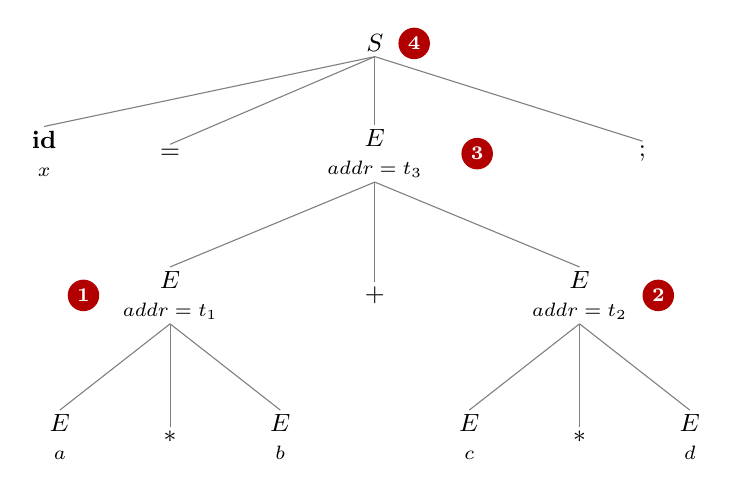
\begin{tikzpicture}[
  every node/.style={font=\small},
  nd/.style={inner sep=1.5pt,align=center},
  no/.style={circle,fill=red!70!black,text=white,inner sep=1pt,minimum size=4mm,font=\scriptsize\bfseries}]
 \node[nd] (S)  at (0,0) {$S$};
 \node[nd] (id) at (-4.2,-1.4) {\textbf{id}\\[-1pt]{\scriptsize $x$}};
 \node[nd] (eq) at (-2.6,-1.4) {$=$};
 \node[nd] (E)  at (0,-1.4) {$E$\\[-1pt]{\scriptsize $addr=t_3$}};
 \node[nd] (sc) at (3.4,-1.4) {$;$};
 \node[nd] (E1) at (-2.6,-3.2) {$E$\\[-1pt]{\scriptsize $addr=t_1$}};
 \node[nd] (pl) at (0,-3.2) {$+$};
 \node[nd] (E2) at (2.6,-3.2) {$E$\\[-1pt]{\scriptsize $addr=t_2$}};
 \node[nd] (a) at (-4.0,-5) {$E$\\[-1pt]{\scriptsize $a$}};
 \node[nd] (m1) at (-2.6,-5) {$*$};
 \node[nd] (b) at (-1.2,-5) {$E$\\[-1pt]{\scriptsize $b$}};
 \node[nd] (c) at (1.2,-5) {$E$\\[-1pt]{\scriptsize $c$}};
 \node[nd] (m2) at (2.6,-5) {$*$};
 \node[nd] (d) at (4.0,-5) {$E$\\[-1pt]{\scriptsize $d$}};
 \foreach \a/\b in {S/id,S/eq,S/E,S/sc,E/E1,E/pl,E/E2,E1/a,E1/m1,E1/b,E2/c,E2/m2,E2/d}
   \draw[gray] (\a.south)--(\b.north);
 \node[no] at (-3.7,-3.2) {1};
 \node[no] at (3.6,-3.2) {2};
 \node[no] at (1.3,-1.4) {3};
 \node[no] at (0.5,0) {4};
\end{tikzpicture}
\caption{Parse tree of \texttt{x = a * b + c * d ;} with the order of emission.}
\end{figure}

\begin{center}
\small
\begin{tabular}{@{}c l l@{}}
\toprule
\textbf{\#} & \textbf{Reduction} & \textbf{Instruction emitted} \\ \midrule
1 & $E\to E_1*E_2$ \ (\texttt{a * b}) & \texttt{t1 = a * b} \\
2 & $E\to E_1*E_2$ \ (\texttt{c * d}) & \texttt{t2 = c * d} \\
3 & $E\to E_1+E_2$ & \texttt{t3 = t1 + t2} \\
4 & $S\to\mathbf{id}=E\,;$ & \texttt{x = t3} \\ \bottomrule
\end{tabular}
\end{center}
Note that \texttt{c * d} is reduced only after the parser has seen the \texttt{;}: precedence decides that $*$ binds tighter, so the $+$ cannot be reduced earlier.
\end{examplebox}

\subsection{Addressing array elements}
Let an array be stored in a contiguous block of memory with base address $\mathit{base}$ and element width $w$.

\paragraph{One-dimensional array} $A[\mathit{low}\ \dots\ \mathit{high}]$:
\[
\text{address of } A[i] \;=\; \mathit{base} + (i - \mathit{low}) \times w
\]
If $\mathit{low}=0$ this is simply $\mathit{base} + i \times w$.

\paragraph{Two-dimensional array} (row-major) $A[n_1][n_2]$ with element width $w$:
\[
\text{address of } A[i_1][i_2] \;=\; \mathit{base} + (i_1 \times n_2 + i_2) \times w
\]
\paragraph{$k$ dimensions} $A[n_1]\cdots[n_k]$ (row-major, 0-based):
\[
\mathit{base} + \bigl( (\cdots((i_1 n_2 + i_2) n_3 + i_3) \cdots ) n_k + i_k \bigr)\times w
\]
Equivalently, using the \emph{widths of sub-arrays} $w_1 = n_2 \cdots n_k \cdot w,\ w_2 = n_3\cdots n_k \cdot w, \dots,\ w_k = w$:
\[
\mathit{base} + i_1 \times w_1 + i_2 \times w_2 + \cdots + i_k \times w_k.
\]
This form is the one used in the translation scheme.

\begin{figure}[htbp]
\centering
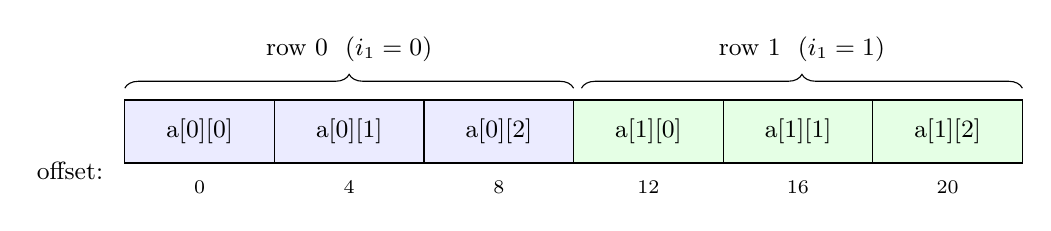
\begin{tikzpicture}[
  cell/.style={draw,minimum width=1.9cm,minimum height=0.8cm,font=\small}]
 \foreach \i/\n/\o in {0/a[0][0]/0, 1/a[0][1]/4, 2/a[0][2]/8, 3/a[1][0]/12, 4/a[1][1]/16, 5/a[1][2]/20} {
   \node[cell,fill=blue!8] at (\i*1.9,0) {\n};
   \node[font=\scriptsize,below] at (\i*1.9,-0.5) {\o};
 }
 \foreach \i in {3,4,5} \node[cell,fill=green!10] at (\i*1.9,0) {};
 \foreach \i/\n in {3/a[1][0],4/a[1][1],5/a[1][2]} \node[font=\small] at (\i*1.9,0) {\n};
 \draw[decorate,decoration={brace,amplitude=5pt}] (-0.95,0.55)--(4.75,0.55) node[midway,above=6pt,font=\small]{row 0 \ ($i_1=0$)};
 \draw[decorate,decoration={brace,amplitude=5pt}] (4.85,0.55)--(10.45,0.55) node[midway,above=6pt,font=\small]{row 1 \ ($i_1=1$)};
 \node[font=\small,anchor=east] at (-1.1,-0.5) {offset:};
\end{tikzpicture}
\caption{Row-major layout of \texttt{int a[2][3]} ($w=4$). Offset of $a[i][j]$ is $i\times 12 + j\times 4$.}
\end{figure}

\subsection{Translation of array references}
Grammar (with nonterminal $L$ for an array location):
\begin{align*}
S &\to \mathbf{id} = E\ ;\ \mid\ L = E\ ;\\
E &\to E_1 + E_2\ \mid\ \mathbf{id}\ \mid\ L\\
L &\to \mathbf{id}\,[\,E\,]\ \mid\ L_1\,[\,E\,]
\end{align*}
Attributes of $L$: \at{L}{array} (symbol-table entry of the array), \at{L}{type} (type of the \emph{sub-array} generated by $L$), \at{L}{addr} (a temporary accumulating the \emph{offset}).

\begin{table}[htbp]
\centering
\small
\begin{tabular}{@{}L{2.4cm} L{12.2cm}@{}}
\toprule
\textbf{Production} & \textbf{Semantic action} \\ \midrule
$S \to \mathbf{id}=E\ ;$ & $\{\ \mathit{gen}(\mathit{top}.\mathit{get}(\at{\mathbf{id}}{lexeme})\ \tok{=}\ \at{E}{addr});\ \}$ \\[2pt]
$S \to L=E\ ;$ & $\{\ \mathit{gen}(\at{L}{array}.\mathit{base}\ \tok{[}\ \at{L}{addr}\ \tok{]}\ \tok{=}\ \at{E}{addr});\ \}$ \\[2pt]
$E \to E_1+E_2$ & $\{\ \at{E}{addr}=\mathbf{new}\ \mathit{Temp}();\ \mathit{gen}(\at{E}{addr}\ \tok{=}\ \at{E_1}{addr}\ \tok{+}\ \at{E_2}{addr});\ \}$ \\[2pt]
$E \to \mathbf{id}$ & $\{\ \at{E}{addr}=\mathit{top}.\mathit{get}(\at{\mathbf{id}}{lexeme});\ \}$ \\[2pt]
$E \to L$ & $\{\ \at{E}{addr}=\mathbf{new}\ \mathit{Temp}();\ \mathit{gen}(\at{E}{addr}\ \tok{=}\ \at{L}{array}.\mathit{base}\ \tok{[}\ \at{L}{addr}\ \tok{]});\ \}$ \\[2pt]
$L \to \mathbf{id}\,[\,E\,]$ & $\{\ \at{L}{array}=\mathit{top}.\mathit{get}(\at{\mathbf{id}}{lexeme});\ \at{L}{type}=\at{L}{array}.\mathit{type}.\mathit{elem};$\\
 & $\ \ \at{L}{addr}=\mathbf{new}\ \mathit{Temp}();\ \mathit{gen}(\at{L}{addr}\ \tok{=}\ \at{E}{addr}\ \tok{*}\ \at{L}{type}.\mathit{width});\ \}$ \\[2pt]
$L \to L_1\,[\,E\,]$ & $\{\ \at{L}{array}=\at{L_1}{array};\ \at{L}{type}=\at{L_1}{type}.\mathit{elem};$\\
 & $\ \ t=\mathbf{new}\ \mathit{Temp}();\ \at{L}{addr}=\mathbf{new}\ \mathit{Temp}();$\\
 & $\ \ \mathit{gen}(t\ \tok{=}\ \at{E}{addr}\ \tok{*}\ \at{L}{type}.\mathit{width});\ \mathit{gen}(\at{L}{addr}\ \tok{=}\ \at{L_1}{addr}\ \tok{+}\ t);\ \}$ \\ \bottomrule
\end{tabular}
\caption{Semantic actions for array references (Dragon Book Fig.~6.22).}
\end{table}

\begin{examplebox}{Worked example: $c + a[i][j]$ where \texttt{a} is \texttt{int a[2][3]}}
Types: \at{a}{type} $= \mathit{array}(2,\ \mathit{array}(3,\ \mathit{integer}))$, so the width of one row is $3\times 4 = 12$ and of an element is $4$.

\begin{enumerate}[nosep]
\item $L \to \mathbf{id}[E]$ with $E = i$: $\at{L}{type}=\mathit{array}(3,\mathit{integer})$, width 12 \;$\Rightarrow$\; \texttt{t1 = i * 12}.
\item $L \to L_1[E]$ with $E = j$: $\at{L}{type}=\mathit{integer}$, width 4 \;$\Rightarrow$\; \texttt{t2 = j * 4}, \texttt{t3 = t1 + t2}.
\item $E \to L$: \texttt{t4 = a[t3]}.
\item $E \to E_1 + E_2$: \texttt{t5 = c + t4}.
\end{enumerate}
\begin{lstlisting}
t1 = i * 12
t2 = j * 4
t3 = t1 + t2
t4 = a[t3]
t5 = c + t4
\end{lstlisting}

And for the assignment $x = a[i][j]$ the code is the first four instructions followed by \texttt{x = t4}.
\end{examplebox}

\begin{examplebox}{Worked example: a three-dimensional array and a store}
Let \texttt{int a[2][3][4]} (so $w=4$). The widths of the sub-arrays are $w_3=4$ (one element), $w_2=4\cdot4=16$ (one innermost row of 4 elements) and $w_1=3\cdot4\cdot4=48$ (one $3\times4$ plane); the whole array occupies $2\cdot48=96$ bytes. The statement \texttt{x = a[i][j][k];} becomes
\begin{lstlisting}
t1 = i * 48
t2 = j * 16
t3 = t1 + t2
t4 = k * 4
t5 = t3 + t4
t6 = a[t5]
x  = t6
\end{lstlisting}
Each extra subscript adds exactly two instructions (a multiplication and an addition), as in the rule for $L\to L_1[E]$. For a \emph{store}, \texttt{a[i][j] = x;} with \texttt{int a[2][3]} uses the rule $S\to L=E\,;$, which ends with an indexed assignment instead of an indexed load:
\begin{lstlisting}
t1 = i * 12
t2 = j * 4
t3 = t1 + t2
a[t3] = x
\end{lstlisting}
\end{examplebox}

\begin{pitfallbox}{Index versus offset}
In \texttt{t4 = a[t3]} the value in \texttt{t3} is a \emph{byte offset} from the base of \texttt{a}, not an element index as in the C source. That is why every subscript is multiplied by the width of the thing it selects. (In the book's three-address code, \texttt{x = y[i]} means ``the value at the memory location $i$ units beyond $y$''.)
\end{pitfallbox}

%====================================================================
\section{Type Checking and Type Conversion}
%====================================================================

\paragraph{Type expressions} represent the type of a language construct: basic types (\texttt{int}, \texttt{float}, \texttt{char}, \texttt{boolean}, \texttt{void}), \textit{array}$(n, T)$, \textit{record}, pointer, and function types $s \to t$.

\paragraph{Type checking} comes in two forms: \textbf{synthesis} (the type of an expression is built from the types of its sub-expressions, e.g., for $E_1 + E_2$) and \textbf{inference} (the type of a construct is determined from the way it is used).

\begin{examplebox}{Example: three static checks}
Static checking attaches a rule to a production and reports an error when the rule fails. With \texttt{int a[10]; int n; float f;}:
\begin{center}
\small
\begin{tabular}{@{}l L{5.6cm} L{4.6cm}@{}}
\toprule
\textbf{Source} & \textbf{Rule that fails} & \textbf{Message} \\ \midrule
\texttt{x = a[2.5];} & in $L\to\mathbf{id}[E]$ the index $E$ must have type \texttt{int} & array index must be an integer \\
\texttt{y = a + n;} & $+$ is defined for numeric types only; $a$ has type $\mathit{array}(10,\texttt{int})$ & operand of $+$ is not a number \\
\texttt{if (f) x = 1;} & the condition in \texttt{if (}$E$\texttt{)} must have type \texttt{boolean} & \texttt{float} used as condition (C would accept it and test $f\ne0$) \\ \bottomrule
\end{tabular}
\end{center}
Each check is just one more semantic rule: it computes nothing, it only compares attribute values and calls an error routine, which is another example of a rule with a side effect.
\end{examplebox}

\subsection{Type conversion (coercion)}
For $E \to E_1 + E_2$ where operand types may differ (e.g., \texttt{int} and \texttt{float}), the compiler inserts conversions. Conversions that cannot lose information in principle (\emph{widening}) may be inserted by the compiler automatically (\emph{coercion}); the reverse direction (\emph{narrowing}) needs an explicit cast written by the programmer. Figure~\ref{fig:typehier} shows the usual hierarchy. In these notes we use only \texttt{int} $<$ \texttt{float}.
\begin{figure}[H]
\centering
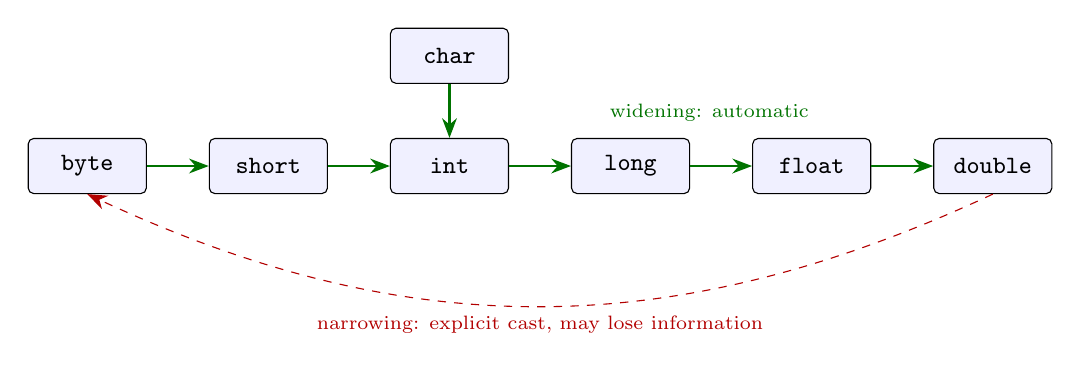
\begin{tikzpicture}[
  t/.style={draw,rounded corners=2pt,minimum width=1.5cm,minimum height=0.7cm,font=\small\ttfamily,fill=blue!6},
  wide/.style={-{Stealth[length=2.5mm]},thick,green!45!black},
  narrow/.style={-{Stealth[length=2.5mm]},dashed,red!70!black}]
 \node[t] (by) at (0,0) {byte};
 \node[t] (sh) at (2.3,0) {short};
 \node[t] (in) at (4.6,0) {int};
 \node[t] (lo) at (6.9,0) {long};
 \node[t] (fl) at (9.2,0) {float};
 \node[t] (do) at (11.5,0) {double};
 \node[t] (ch) at (4.6,1.4) {char};
 \foreach \a/\b in {by/sh,sh/in,in/lo,lo/fl,fl/do} \draw[wide] (\a)--(\b);
 \draw[wide] (ch)--(in);
 \draw[narrow] (do.south) to[bend left=25] node[below,font=\scriptsize]{narrowing: explicit cast, may lose information} (by.south);
 \node[font=\scriptsize,green!45!black,anchor=south] at (7.9,0.45) {widening: automatic};
\end{tikzpicture}
\caption{Widening (solid) and narrowing (dashed) conversions between primitive types, Java-style. Converting \texttt{long} to \texttt{float} is allowed implicitly although a few low-order digits may be rounded.}
\label{fig:typehier}
\end{figure}
For $E \to E_1 + E_2$ (and likewise for $-$, $*$, $/$) the result has the \emph{wider} of the two operand types,
\[
\at{E}{type} = \max(\at{E_1}{type},\ \at{E_2}{type}),
\]
and the helper $\mathit{widen}(a, t, w)$ converts address $a$ of type $t$ to type $w$:

\begin{lstlisting}
Addr widen(Addr a, Type t, Type w) {
    if (t == w) return a;
    else if (t == integer && w == float) {
        temp = new Temp();
        gen(temp '=' '(float)' a);
        return temp;
    }
    else error;
}
\end{lstlisting}

\begin{center}
\small
\begin{tabular}{@{}L{3.1cm} L{11.4cm}@{}}
\toprule
\textbf{Production} & \textbf{Semantic action} \\ \midrule
$E \to E_1 + E_2$ &
$\{\ \at{E}{type}=\max(\at{E_1}{type},\at{E_2}{type});$\\
& $\ \ a_1=\mathit{widen}(\at{E_1}{addr},\at{E_1}{type},\at{E}{type});$\\
& $\ \ a_2=\mathit{widen}(\at{E_2}{addr},\at{E_2}{type},\at{E}{type});$\\
& $\ \ \at{E}{addr}=\mathbf{new}\ \mathit{Temp}();\ \mathit{gen}(\at{E}{addr}\ \tok{=}\ a_1\ \tok{+}\ a_2);\ \}$ \\ \bottomrule
\end{tabular}
\end{center}

\begin{examplebox}{Example}
Let \texttt{x} be \texttt{float}, and \texttt{i, j} be \texttt{int}. For $x = i * j + x$ we get:
\begin{lstlisting}
t1 = i * j          // int * int -> int
t2 = (float) t1     // widen to float
t3 = t2 + x         // float + float
x  = t3
\end{lstlisting}
\end{examplebox}

\begin{examplebox}{Worked example: widening on \emph{both} sides, $x = i + j * x$}
Let \texttt{x} be \texttt{float} and \texttt{i, j} be \texttt{int}. The code is emitted at reductions, so the product $j*x$ (reduced first) comes before the sum:
\begin{enumerate}[nosep]
\item $E\to E_1*E_2$ with $E_1=j$ (\texttt{int}) and $E_2=x$ (\texttt{float}): $E.type=\texttt{float}$; $\mathit{widen}(j)$ emits \texttt{t1 = (float) j}; $\mathit{widen}(x)$ does nothing; then \texttt{t2 = t1 * x}.
\item $E\to E_1+E_2$ with $E_1=i$ (\texttt{int}) and $E_2$ of type \texttt{float}: $\mathit{widen}(i)$ emits \texttt{t3 = (float) i}; then \texttt{t4 = t3 + t2}.
\item $S\to\mathbf{id}=E\,;$ emits \texttt{x = t4}.
\end{enumerate}
\begin{lstlisting}
t1 = (float) j
t2 = t1 * x
t3 = (float) i
t4 = t3 + t2
x  = t4
\end{lstlisting}
Note that $i$, which is written first, is converted \emph{after} $j$: the order of the instructions follows the order of the reductions, not the order of the source text.
\end{examplebox}

%====================================================================
\section{Control Flow: Boolean Expressions and Statements}
%====================================================================

In programming languages, boolean expressions are used for two purposes:
\begin{enumerate}[nosep]
\item to \textbf{compute logical values} (e.g., \texttt{flag = a < b \&\& c;}), and
\item as \textbf{conditional expressions} in \texttt{if}, \texttt{while}, and \texttt{for} (flow-of-control).
\end{enumerate}
We use the grammar
\[
B \to B \,|\!|\, B \ \mid\ B\ \&\&\ B\ \mid\ !\,B\ \mid\ (B)\ \mid\ E\ \mathit{rel}\ E\ \mid\ \mathbf{true}\ \mid\ \mathbf{false}
\]
with $|\!|$ standing for the C operator \texttt{||}; \texttt{||} and \texttt{\&\&} are left-associative, \texttt{||} has lower precedence than \texttt{\&\&}, which is lower than \texttt{!}.

\subsection{Short-circuit (jumping) code}
In \textbf{short-circuit code}, the operators \texttt{\&\&}, \texttt{||} and \texttt{!} do not appear in the generated code. Instead a boolean expression is translated into jumps to labels: control \emph{reaches} one position if the expression is true and another if it is false. In
\[
\texttt{if (x < 100 || x > 200 \&\& x != y) x = 0;}
\]
the first test \texttt{x<100} being true makes the other tests unnecessary. The generated code is:

\begin{lstlisting}
        if x < 100 goto L2
        goto L3
L3:     if x > 200 goto L4
        goto L1
L4:     if x != y goto L2
        goto L1
L2:     x = 0
L1:     ...
\end{lstlisting}
(Compare with \emph{value} code, which would compute 0/1 into temporaries and use \texttt{\&\&} and \texttt{||} at run time.)

\begin{figure}[H]
\centering
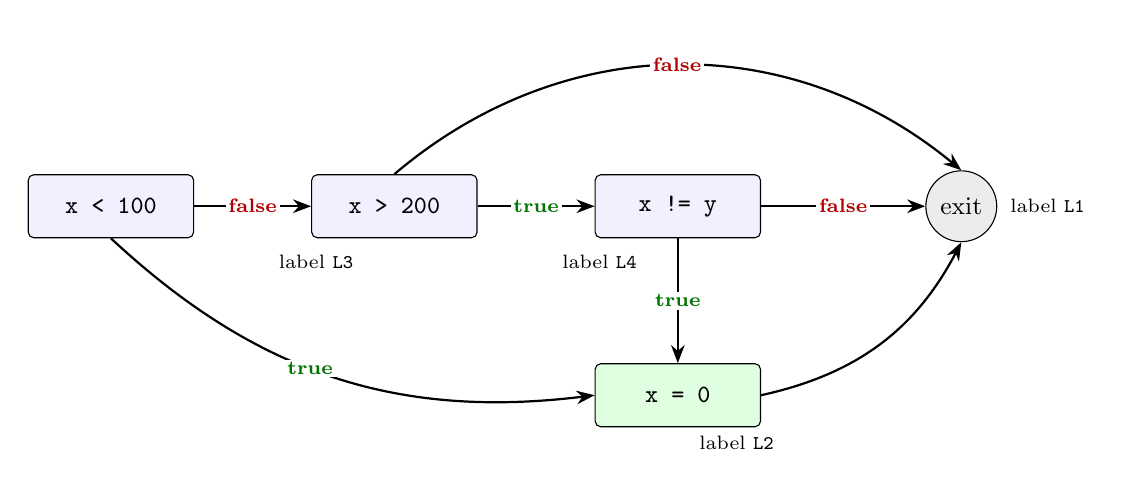
\begin{tikzpicture}[
  every node/.style={font=\small},
  t/.style={draw,rounded corners=2pt,minimum width=2.1cm,minimum height=0.8cm,fill=blue!6,font=\small\ttfamily},
  o/.style={draw,rounded corners=2pt,minimum width=2.1cm,minimum height=0.8cm,fill=green!12,font=\small\ttfamily},
  e/.style={-{Stealth[length=2.3mm]},thick},
  yes/.style={font=\scriptsize\bfseries,text=green!45!black,fill=white,inner sep=1pt},
  no/.style={font=\scriptsize\bfseries,text=red!70!black,fill=white,inner sep=1pt}]
 \node[t] (a) at (0,0) {x < 100};
 \node[t] (b) at (3.6,0) {x > 200};
 \node[t] (c) at (7.2,0) {x != y};
 \node[o] (s) at (7.2,-2.4) {x = 0};
 \node[draw,circle,minimum size=0.9cm,fill=gray!15,font=\small] (x) at (10.8,0) {exit};
 \draw[e] (a) -- node[no]{false} (b);
 \draw[e] (b) -- node[yes]{true} (c);
 \draw[e] (c) -- node[no]{false} (x);
 \draw[e] (c) -- node[yes]{true} (s);
 \draw[e] (a.south) to[bend right=25] node[yes,pos=0.45]{true} (s.west);
 \draw[e] (b.north) to[bend left=40] node[no,pos=0.5]{false} (x.north);
 \draw[e] (s.east) to[bend right=25] (x.south);
 \node[font=\scriptsize,anchor=east] at (3.2,-0.7) {label \texttt{L3}};
 \node[font=\scriptsize,anchor=east] at (6.8,-0.7) {label \texttt{L4}};
 \node[font=\scriptsize,anchor=west] at (7.35,-3.0) {label \texttt{L2}};
 \node[font=\scriptsize,anchor=west] at (11.3,0) {label \texttt{L1}};
\end{tikzpicture}
\caption{Control-flow view of \texttt{if (x < 100 || x > 200 \&\& x != y) x = 0;}. Each test jumps on its own outcome; no boolean value is ever computed. A \emph{true} arrow out of $x<100$ skips the other tests.}
\end{figure}

\begin{pitfallbox}{Short-circuit evaluation is a semantic guarantee, not only an optimisation}
In \texttt{if (p != NULL \&\& p->x > 0) \dots} the second operand must \emph{not} be evaluated when $p$ is null, otherwise the program dereferences a null pointer. Jumping code gives this behaviour for free: the test of \texttt{p->x} is only reached through the \emph{true} exit of \texttt{p != NULL}. Value code that first computes both operands would crash.
\end{pitfallbox}

\paragraph{Boolean values in assignments.} A boolean expression is also used to compute a \emph{value}, e.g.\ \texttt{flag = a < b \&\& c;}. The jumping code is reused, and the two exits set the variable:
\begin{lstlisting}
        if a < b goto L1
        goto L3
L1:     if c goto L2
        goto L3
L2:     flag = true
        goto L4
L3:     flag = false
L4:
\end{lstlisting}

\subsection{Flow-of-control statements: SDD with inherited labels}
Grammar for statements:
\[
P \to S, \qquad S \to \mathbf{assign}\ \mid\ \mathbf{if}\,(B)\,S_1\ \mid\ \mathbf{if}\,(B)\,S_1\ \mathbf{else}\ S_2\ \mid\ \mathbf{while}\,(B)\,S_1\ \mid\ S_1\,S_2
\]
\textbf{Inherited attributes} (labels):
\begin{itemize}
\item \at{B}{true}: the label to jump to if $B$ is true; \at{B}{false}: the label if $B$ is false.
\item \at{S}{next}: the label of the instruction that follows the code for $S$.
\end{itemize}
\textbf{Synthesized attribute}: \at{S}{code}, \at{B}{code}. The function $\mathit{newlabel}()$ creates a fresh label $L_1, L_2, \dots$, and $\lbl{L}$ attaches label $L$ to the next instruction.

\begin{table}[htbp]
\centering
\small
\begin{tabular}{@{}L{3.6cm} L{11cm}@{}}
\toprule
\textbf{Production} & \textbf{Semantic rules} \\ \midrule
$P \to S$ &
$\at{S}{next}=\mathit{newlabel}()$;\quad $\at{P}{code}=\at{S}{code}\cc\lbl{\at{S}{next}}$ \\[3pt]
$S \to \mathbf{assign}$ &
$\at{S}{code}=\at{\mathbf{assign}}{code}$ \\[3pt]
$S \to \mathbf{if}\,(B)\,S_1$ &
$\at{B}{true}=\mathit{newlabel}()$;\quad $\at{B}{false}=\at{S_1}{next}=\at{S}{next}$\\
& $\at{S}{code}=\at{B}{code}\cc\lbl{\at{B}{true}}\cc\at{S_1}{code}$ \\[3pt]
$S \to \mathbf{if}\,(B)\,S_1\ \mathbf{else}\ S_2$ &
$\at{B}{true}=\mathit{newlabel}()$;\quad $\at{B}{false}=\mathit{newlabel}()$;\quad $\at{S_1}{next}=\at{S_2}{next}=\at{S}{next}$\\
& $\at{S}{code}=\at{B}{code}\cc\lbl{\at{B}{true}}\cc\at{S_1}{code}\cc\gen{\goto\ \at{S}{next}}\cc\lbl{\at{B}{false}}\cc\at{S_2}{code}$ \\[3pt]
$S \to \mathbf{while}\,(B)\,S_1$ &
$\mathit{begin}=\mathit{newlabel}()$;\quad $\at{B}{true}=\mathit{newlabel}()$;\quad $\at{B}{false}=\at{S}{next}$;\quad $\at{S_1}{next}=\mathit{begin}$\\
& $\at{S}{code}=\lbl{\mathit{begin}}\cc\at{B}{code}\cc\lbl{\at{B}{true}}\cc\at{S_1}{code}\cc\gen{\goto\ \mathit{begin}}$ \\[3pt]
$S \to S_1\,S_2$ &
$\at{S_1}{next}=\mathit{newlabel}()$;\quad $\at{S_2}{next}=\at{S}{next}$\\
& $\at{S}{code}=\at{S_1}{code}\cc\lbl{\at{S_1}{next}}\cc\at{S_2}{code}$ \\ \bottomrule
\end{tabular}
\caption{SDD for flow-of-control statements (Dragon Book Fig.~6.36). \at{S}{next}, \at{B}{true}, and \at{B}{false} are inherited.}
\end{table}

\begin{figure}[htbp]
\centering
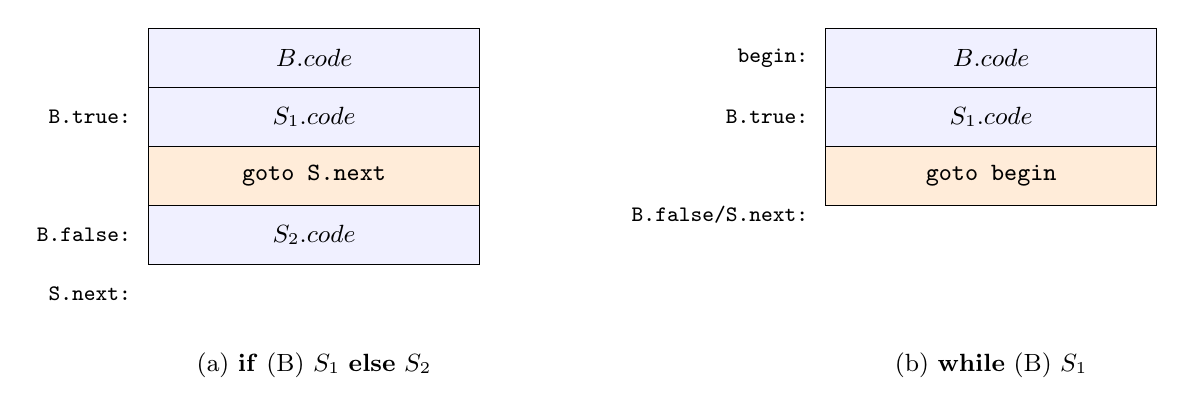
\begin{tikzpicture}[
  blk/.style={draw,minimum width=4.2cm,minimum height=0.75cm,font=\small,fill=blue!6},
  lab/.style={font=\footnotesize\ttfamily,anchor=east}]
 % if-else
 \node[blk] (b) at (0,0) {$B.code$};
 \node[blk] (s1) at (0,-0.75) {$S_1.code$};
 \node[blk,fill=orange!15] (g) at (0,-1.5) {\texttt{goto S.next}};
 \node[blk] (s2) at (0,-2.25) {$S_2.code$};
 \node[lab] at (-2.2,-0.75) {B.true:};
 \node[lab] at (-2.2,-2.25) {B.false:};
 \node[lab] at (-2.2,-3.0) {S.next:};
 \node[font=\small] at (0,-3.9) {(a) \textbf{if} (B) $S_1$ \textbf{else} $S_2$};
 % while
 \begin{scope}[xshift=8.6cm]
 \node[blk] (wb) at (0,0) {$B.code$};
 \node[blk] (ws) at (0,-0.75) {$S_1.code$};
 \node[blk,fill=orange!15] (wg) at (0,-1.5) {\texttt{goto begin}};
 \node[lab] at (-2.2,0) {begin:};
 \node[lab] at (-2.2,-0.75) {B.true:};
 \node[lab] at (-2.2,-2.0) {B.false/S.next:};
 \node[font=\small] at (0,-3.9) {(b) \textbf{while} (B) $S_1$};
 \end{scope}
\end{tikzpicture}
\caption{Layout of the generated code. $B.code$ contains jumps to \textit{B.true} or \textit{B.false}; it ``falls through'' to neither, so the labels can be placed anywhere.}
\end{figure}

\subsection{SDD for boolean expressions (jumping code)}
\begin{table}[htbp]
\centering
\small
\begin{tabular}{@{}L{3.1cm} L{11.5cm}@{}}
\toprule
\textbf{Production} & \textbf{Semantic rules} \\ \midrule
$B \to B_1 \,|\!|\, B_2$ &
$\at{B_1}{true}=\at{B}{true}$;\ \ $\at{B_1}{false}=\mathit{newlabel}()$;\ \ $\at{B_2}{true}=\at{B}{true}$;\ \ $\at{B_2}{false}=\at{B}{false}$\\
& $\at{B}{code}=\at{B_1}{code}\cc\lbl{\at{B_1}{false}}\cc\at{B_2}{code}$ \\[3pt]
$B \to B_1\ \&\&\ B_2$ &
$\at{B_1}{true}=\mathit{newlabel}()$;\ \ $\at{B_1}{false}=\at{B}{false}$;\ \ $\at{B_2}{true}=\at{B}{true}$;\ \ $\at{B_2}{false}=\at{B}{false}$\\
& $\at{B}{code}=\at{B_1}{code}\cc\lbl{\at{B_1}{true}}\cc\at{B_2}{code}$ \\[3pt]
$B \to !\,B_1$ &
$\at{B_1}{true}=\at{B}{false}$;\ \ $\at{B_1}{false}=\at{B}{true}$;\ \ $\at{B}{code}=\at{B_1}{code}$ \\[3pt]
$B \to E_1\ \mathit{rel}\ E_2$ &
$\at{B}{code}=\at{E_1}{code}\cc\at{E_2}{code}\cc\gen{\mathbf{if}\ \at{E_1}{addr}\ \mathit{rel.op}\ \at{E_2}{addr}\ \goto\ \at{B}{true}}\cc\gen{\goto\ \at{B}{false}}$ \\[3pt]
$B \to \mathbf{true}$ & $\at{B}{code}=\gen{\goto\ \at{B}{true}}$ \\[3pt]
$B \to \mathbf{false}$ & $\at{B}{code}=\gen{\goto\ \at{B}{false}}$ \\ \bottomrule
\end{tabular}
\caption{SDD to generate jumping code for boolean expressions (Dragon Book Fig.~6.37).}
\end{table}

\begin{notebox}{How to remember the \texttt{||} and \texttt{\&\&} rules}
\begin{itemize}[nosep]
\item $B_1 \,||\, B_2$: if $B_1$ is true we are done (go to \textit{B.true}); if false, \emph{test $B_2$}, so $B_1.\mathit{false}$ is a new label placed in front of $B_2.\mathit{code}$.
\item $B_1 \,\&\&\, B_2$: if $B_1$ is false we are done (go to \textit{B.false}); if true, \emph{test $B_2$}, so $B_1.\mathit{true}$ is a new label in front of $B_2.\mathit{code}$.
\item $!\,B_1$: simply \emph{swap} the true and false labels.
\end{itemize}
\end{notebox}

\begin{examplebox}{Worked example: \texttt{if (x < 100 || x > 200 \&\& x != y) x = 0;}}
\textbf{Step 1.} $P \to S$: \at{S}{next} $= L_1$.

\textbf{Step 2.} $S \to \mathbf{if}(B)S_1$: \at{B}{true} $= L_2$, \at{B}{false} $= L_1$, \at{S_1}{next} $= L_1$.

\textbf{Step 3.} $B = B_1 \,||\, B_2$, where $B_1 \equiv x<100$ and $B_2 \equiv (x>200 \;\&\&\; x\ne y)$:
\begin{itemize}[nosep]
\item $B_1$: true $= L_2$, false $= L_3$ (new).
\item $B_2$: true $= L_2$, false $= L_1$.
\end{itemize}
\textbf{Step 4.} $B_2 = B_3 \,\&\&\, B_4$ with $B_3 \equiv x>200$, $B_4 \equiv x \ne y$:
\begin{itemize}[nosep]
\item $B_3$: true $= L_4$ (new), false $= L_1$.
\item $B_4$: true $= L_2$, false $= L_1$.
\end{itemize}
\textbf{Step 5.} Assemble: $B_1.code \cc L_3{:}\ B_2.code$, with $B_2.code = B_3.code \cc L_4{:}\ B_4.code$, followed by $L_2{:}\ S_1.code$ and finally $L_1{:}$

\begin{lstlisting}
        if x < 100 goto L2
        goto L3
L3:     if x > 200 goto L4
        goto L1
L4:     if x != y goto L2
        goto L1
L2:     x = 0
L1:
\end{lstlisting}
Observe the redundant jumps (\texttt{goto L3} immediately followed by \texttt{L3:}) -- a later optimisation phase or the \emph{backpatching} method with fall-through can remove them.
\end{examplebox}

\begin{examplebox}{Worked example: \texttt{while (a < b) \{ if (c < d) x = y + z; \}}}
\begin{lstlisting}
L1:     if a < b goto L2        // begin / B.code
        goto L0                 // B.false = S.next
L2:     if c < d goto L3        // inner if: B.true = L3
        goto L1                 // inner S.next = begin = L1
L3:     t1 = y + z
        x = t1
        goto L1                 // goto begin
L0:                             // S.next
\end{lstlisting}
\end{examplebox}

\subsection{Avoiding redundant gotos (fall-through)}
Instead of
\begin{lstlisting}
        if x > 200 goto L4
        goto L1
L4:     ...
\end{lstlisting}
we can generate the shorter form \texttt{ifFalse x > 200 goto L1} followed by the code at \texttt{L4}: if the true label is the next instruction (denote it by the special label \textit{fall}), only one jump is needed. The rule for $B \to E_1\ \mathit{rel}\ E_2$ becomes: let $\mathit{test} = E_1.addr\ rel.op\ E_2.addr$:
\begin{center}
\small
\begin{tabular}{@{}l l@{}}
\toprule
\textbf{Condition} & \textbf{Generated jump code} \\ \midrule
\at{B}{true}\ $\ne$ \textit{fall} and \at{B}{false}\ $\ne$ \textit{fall} & \texttt{if test goto B.true} \quad \texttt{goto B.false} \\
\at{B}{true}\ $\ne$ \textit{fall} and \at{B}{false} = \textit{fall} & \texttt{if test goto B.true} \\
\at{B}{true} = \textit{fall} and \at{B}{false}\ $\ne$ \textit{fall} & \texttt{ifFalse test goto B.false} \\
both = \textit{fall} & (no instruction) \\ \bottomrule
\end{tabular}
\end{center}

\paragraph{The statement and operator rules change too.} Let \textit{fall} mean ``the next instruction in sequence''. The new rules (Dragon Book Section 6.6.5) are:
\begin{center}
\small
\begin{tabular}{@{}L{2.9cm} L{11.7cm}@{}}
\toprule
\textbf{Production} & \textbf{Semantic rules} \\ \midrule
$S\to\mathbf{if}\,(B)\,S_1$ & $\at{B}{true}=\textit{fall}$;\ \ $\at{B}{false}=\at{S_1}{next}=\at{S}{next}$;\ \ $\at{S}{code}=\at{B}{code}\cc\at{S_1}{code}$ \\[3pt]
$B\to B_1\,|\!|\,B_2$ &
$\at{B_1}{true}=$ (\at{B}{true} if $\ne$ \textit{fall}, else a new label);\ \ $\at{B_1}{false}=\textit{fall}$;\ \ $\at{B_2}{true}=\at{B}{true}$;\ \ $\at{B_2}{false}=\at{B}{false}$\\
& $\at{B}{code}=\at{B_1}{code}\cc\at{B_2}{code}$ if $\at{B}{true}\ne\textit{fall}$; otherwise $\at{B_1}{code}\cc\at{B_2}{code}\cc\lbl{\at{B_1}{true}}$ \\[3pt]
$B\to B_1\ \&\&\ B_2$ &
$\at{B_1}{true}=\textit{fall}$;\ \ $\at{B_1}{false}=$ (\at{B}{false} if $\ne$ \textit{fall}, else a new label);\ \ $\at{B_2}{true}=\at{B}{true}$;\ \ $\at{B_2}{false}=\at{B}{false}$\\
& $\at{B}{code}=\at{B_1}{code}\cc\at{B_2}{code}$ if $\at{B}{false}\ne\textit{fall}$; otherwise $\at{B_1}{code}\cc\at{B_2}{code}\cc\lbl{\at{B_1}{false}}$ \\ \bottomrule
\end{tabular}
\end{center}
The extra label in the ``otherwise'' case is needed because when $B_1$ is decisive the control must jump \emph{past} $B_2$, to the end of $B.code$.

\begin{examplebox}{Worked example: the same statement with fall-through}
For \texttt{if (x < 100 || x > 200 \&\& x != y) x = 0;} start with $B.true=\textit{fall}$ and $B.false=L_1$. For $B_1\,||\,B_2$: since $B.true=\textit{fall}$, $B_1.true=L_2$ (new) and $B_1.false=\textit{fall}$; $B_2$ inherits $B.true=\textit{fall}$ and $B.false=L_1$. For $B_2=B_3\,\&\&\,B_4$: $B_3.true=B_4.true=\textit{fall}$ and $B_3.false=B_4.false=L_1$. The relational rule then gives
\begin{lstlisting}
        if x < 100 goto L2
        ifFalse x > 200 goto L1
        ifFalse x != y goto L1
L2:     x = 0
L1:
\end{lstlisting}
Only 4 instructions (3 tests and the assignment) instead of 7, and no useless \texttt{goto}s.
\end{examplebox}

%====================================================================
\section{Backpatching}
\label{sec:backpatch}
%====================================================================

\subsection{The problem and the idea}
In the one-pass, label-based scheme above we needed \emph{inherited} labels (\at{B}{true}, \at{S}{next}) because a jump may be generated \emph{before} its target is known. Inherited attributes make one-pass \textbf{bottom-up} translation awkward. \textbf{Backpatching} avoids this:
\begin{itemize}
\item When a jump is generated, its \emph{target is left blank}.
\item Each such incomplete jump is put on a \textbf{list} of jumps that will eventually go to the same target.
\item When the target address becomes known, the instructions on the list are \emph{patched} (filled in).
\end{itemize}
Thus we only need \emph{synthesized} attributes (lists of instruction indices), and the whole translation can be done in a single bottom-up pass.

\begin{defbox}{Backpatching primitives}
\begin{itemize}
\item $\mathit{makelist}(i)$: create a new list containing only $i$, an index into the instruction array; return a pointer to it.
\item $\mathit{merge}(p_1, p_2)$: concatenate the lists pointed to by $p_1$ and $p_2$; return the merged list.
\item $\mathit{backpatch}(p, i)$: insert $i$ as the target label for each instruction on the list $p$.
\item $\mathit{nextinstr}$: global variable containing the index of the next instruction to be generated. $\mathit{emit}(\dots)$ appends an instruction and increments it.
\end{itemize}
\end{defbox}

\subsection{Boolean expressions}
Synthesized attributes: \at{B}{truelist} (instructions that jump when $B$ is true) and \at{B}{falselist} (when false). A \textbf{marker nonterminal} $M \to \varepsilon$ records the index of the next instruction (\at{M}{instr}).

\begin{table}[htbp]
\centering
\small
\begin{tabular}{@{}L{3.3cm} L{11.3cm}@{}}
\toprule
\textbf{Production} & \textbf{Semantic action} \\ \midrule
$B \to B_1 \,|\!|\, M\ B_2$ &
$\{\ \mathit{backpatch}(\at{B_1}{falselist},\ \at{M}{instr});$\\
& $\ \ \at{B}{truelist}=\mathit{merge}(\at{B_1}{truelist},\ \at{B_2}{truelist});\ \ \at{B}{falselist}=\at{B_2}{falselist};\ \}$ \\[3pt]
$B \to B_1\ \&\&\ M\ B_2$ &
$\{\ \mathit{backpatch}(\at{B_1}{truelist},\ \at{M}{instr});$\\
& $\ \ \at{B}{truelist}=\at{B_2}{truelist};\ \ \at{B}{falselist}=\mathit{merge}(\at{B_1}{falselist},\ \at{B_2}{falselist});\ \}$ \\[3pt]
$B \to !\,B_1$ &
$\{\ \at{B}{truelist}=\at{B_1}{falselist};\ \at{B}{falselist}=\at{B_1}{truelist};\ \}$ \\[3pt]
$B \to (\,B_1\,)$ &
$\{\ \at{B}{truelist}=\at{B_1}{truelist};\ \at{B}{falselist}=\at{B_1}{falselist};\ \}$ \\[3pt]
$B \to E_1\ \mathit{rel}\ E_2$ &
$\{\ \at{B}{truelist}=\mathit{makelist}(\mathit{nextinstr});\ \at{B}{falselist}=\mathit{makelist}(\mathit{nextinstr}+1);$\\
& $\ \ \mathit{emit}(\tok{if}\ \at{E_1}{addr}\ \mathit{rel.op}\ \at{E_2}{addr}\ \tok{goto}\ \_);\ \ \mathit{emit}(\tok{goto}\ \_);\ \}$ \\[3pt]
$B \to \mathbf{true}$ &
$\{\ \at{B}{truelist}=\mathit{makelist}(\mathit{nextinstr});\ \mathit{emit}(\tok{goto}\ \_);\ \}$ \\[3pt]
$B \to \mathbf{false}$ &
$\{\ \at{B}{falselist}=\mathit{makelist}(\mathit{nextinstr});\ \mathit{emit}(\tok{goto}\ \_);\ \}$ \\[3pt]
$M \to \varepsilon$ &
$\{\ \at{M}{instr}=\mathit{nextinstr};\ \}$ \\ \bottomrule
\end{tabular}
\caption{Translation scheme for boolean expressions using backpatching (Dragon Book Fig.~6.43).}
\end{table}

\begin{examplebox}{Worked example: $x < 100 \;||\; x > 200 \;\&\&\; x \ne y$ (instructions start at index 100)}
\textbf{Parse structure:} $B \Rightarrow B_1 \,||\, M_1\, B_2$, where $B_2 \Rightarrow B_3 \,\&\&\, M_2\, B_4$.

\begin{enumerate}[nosep]
\item $B_1 \equiv x<100$: emit \texttt{100: if x<100 goto \_}, \texttt{101: goto \_}\\
 \hspace*{1em} $B_1.truelist=\{100\}$, $B_1.falselist=\{101\}$.
\item $M_1.instr = 102$.
\item $B_3 \equiv x>200$: emit \texttt{102: if x>200 goto \_}, \texttt{103: goto \_}\\
 \hspace*{1em} $B_3.truelist=\{102\}$, $B_3.falselist=\{103\}$.
\item $M_2.instr = 104$.
\item $B_4 \equiv x\ne y$: emit \texttt{104: if x!=y goto \_}, \texttt{105: goto \_}\\
 \hspace*{1em} $B_4.truelist=\{104\}$, $B_4.falselist=\{105\}$.
\item Reduce $B_2 \to B_3 \,\&\&\, M_2\, B_4$:\ \ $\mathit{backpatch}(\{102\},104)$ $\Rightarrow$ instruction 102 becomes \texttt{if x>200 goto 104}.\\
 \hspace*{1em} $B_2.truelist=\{104\}$, $B_2.falselist=\mathit{merge}(\{103\},\{105\})=\{103,105\}$.
\item Reduce $B \to B_1 \,||\, M_1\, B_2$:\ \ $\mathit{backpatch}(\{101\},102)$ $\Rightarrow$ instruction 101 becomes \texttt{goto 102}.\\
 \hspace*{1em} $B.truelist=\mathit{merge}(\{100\},\{104\})=\{100,104\}$, $B.falselist=\{103,105\}$.
\end{enumerate}
\textbf{Result} (still incomplete -- the lists will be patched by the enclosing statement):
\begin{lstlisting}
100:  if x < 100 goto _      <- on truelist
101:  goto 102
102:  if x > 200 goto 104
103:  goto _                 <- on falselist
104:  if x != y goto _       <- on truelist
105:  goto _                 <- on falselist
\end{lstlisting}

\begin{center}
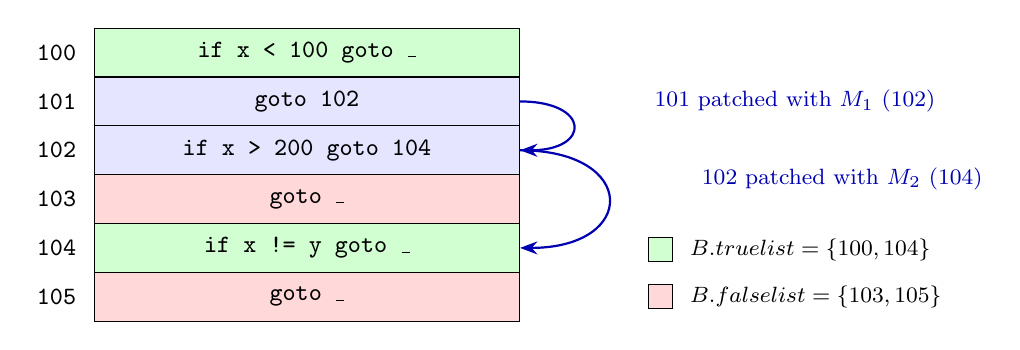
\begin{tikzpicture}[
  every node/.style={font=\small},
  ins/.style={draw,anchor=west,minimum width=5.4cm,minimum height=0.62cm,font=\small\ttfamily},
  idx/.style={font=\small\ttfamily,anchor=east},
  pat/.style={-{Stealth[length=2.2mm]},thick,blue!70!black}]
 \node[idx] at (-0.1,0)     {100};  \node[ins,fill=green!18] (i0) at (0,0)     {if x < 100 goto \_};
 \node[idx] at (-0.1,-0.62) {101};  \node[ins,fill=blue!10]  (i1) at (0,-0.62) {goto 102};
 \node[idx] at (-0.1,-1.24) {102};  \node[ins,fill=blue!10]  (i2) at (0,-1.24) {if x > 200 goto 104};
 \node[idx] at (-0.1,-1.86) {103};  \node[ins,fill=red!15]   (i3) at (0,-1.86) {goto \_};
 \node[idx] at (-0.1,-2.48) {104};  \node[ins,fill=green!18] (i4) at (0,-2.48) {if x != y goto \_};
 \node[idx] at (-0.1,-3.10) {105};  \node[ins,fill=red!15]   (i5) at (0,-3.10) {goto \_};
 \draw[pat] (i1.east) .. controls +(0.9,0) and +(0.9,0) .. (i2.east);
 \draw[pat] (i2.east) .. controls +(1.5,0) and +(1.5,0) .. (i4.east);
 \node[font=\footnotesize,anchor=west,blue!70!black] at (7.0,-0.62) {101 patched with $M_1$ (102)};
 \node[font=\footnotesize,anchor=west,blue!70!black] at (7.6,-1.6) {102 patched with $M_2$ (104)};
 \node[draw,fill=green!18,minimum size=3mm,inner sep=0pt] at (7.2,-2.5) {};
 \node[font=\footnotesize,anchor=west] at (7.45,-2.5) {$B.truelist=\{100,104\}$};
 \node[draw,fill=red!15,minimum size=3mm,inner sep=0pt] at (7.2,-3.1) {};
 \node[font=\footnotesize,anchor=west] at (7.45,-3.1) {$B.falselist=\{103,105\}$};
\end{tikzpicture}
\end{center}
Blue jumps are already complete. The green and red jumps have a blank target; they are exactly the entries of the two lists that the parent will patch.
\end{examplebox}

\subsection{Flow-of-control statements}
Synthesized attribute \at{S}{nextlist}: list of jumps to the instruction that follows $S$. We use markers $M \to \varepsilon$ (records \textit{nextinstr}) and $N \to \varepsilon$ (emits an incomplete \texttt{goto} and returns it on a list).

Grammar:
\begin{align*}
S &\to \mathbf{if}\,(B)\,S_1 \mid \mathbf{if}\,(B)\,S_1\ \mathbf{else}\ S_2 \mid \mathbf{while}\,(B)\,S_1 \mid \{\,L\,\} \mid A\,;\\
L &\to L_1\,S \mid S
\end{align*}
\begin{table}[htbp]
\centering
\small
\begin{tabular}{@{}L{4.3cm} L{10.3cm}@{}}
\toprule
\textbf{Production} & \textbf{Semantic action} \\ \midrule
$S \to \mathbf{if}\,(B)\ M\ S_1$ &
$\{\ \mathit{backpatch}(\at{B}{truelist},\ \at{M}{instr});$\ \ $\at{S}{nextlist}=\mathit{merge}(\at{B}{falselist},\ \at{S_1}{nextlist});\ \}$ \\[3pt]
$S \to \mathbf{if}\,(B)\ M_1\ S_1\ N\ \mathbf{else}\ M_2\ S_2$ &
$\{\ \mathit{backpatch}(\at{B}{truelist},\ \at{M_1}{instr});\ \mathit{backpatch}(\at{B}{falselist},\ \at{M_2}{instr});$\\
& $\ \ \mathit{temp}=\mathit{merge}(\at{S_1}{nextlist},\ \at{N}{nextlist});$\\
& $\ \ \at{S}{nextlist}=\mathit{merge}(\mathit{temp},\ \at{S_2}{nextlist});\ \}$ \\[3pt]
$S \to \mathbf{while}\ M_1\,(B)\ M_2\ S_1$ &
$\{\ \mathit{backpatch}(\at{S_1}{nextlist},\ \at{M_1}{instr});$\\
& $\ \ \mathit{backpatch}(\at{B}{truelist},\ \at{M_2}{instr});$\\
& $\ \ \at{S}{nextlist}=\at{B}{falselist};\ \mathit{emit}(\tok{goto}\ \at{M_1}{instr});\ \}$ \\[3pt]
$S \to \{\ L\ \}$ & $\{\ \at{S}{nextlist}=\at{L}{nextlist};\ \}$ \\[3pt]
$S \to A\ ;$ & $\{\ \at{S}{nextlist}=\mathbf{null};\ \}$ \\[3pt]
$L \to L_1\ M\ S$ & $\{\ \mathit{backpatch}(\at{L_1}{nextlist},\ \at{M}{instr});\ \at{L}{nextlist}=\at{S}{nextlist};\ \}$ \\[3pt]
$L \to S$ & $\{\ \at{L}{nextlist}=\at{S}{nextlist};\ \}$ \\[3pt]
$M \to \varepsilon$ & $\{\ \at{M}{instr}=\mathit{nextinstr};\ \}$ \\[3pt]
$N \to \varepsilon$ & $\{\ \at{N}{nextlist}=\mathit{makelist}(\mathit{nextinstr});\ \mathit{emit}(\tok{goto}\ \_);\ \}$ \\ \bottomrule
\end{tabular}
\caption{Translation of statements with backpatching (Dragon Book Fig.~6.46).}
\end{table}

\begin{notebox}{Why the markers?}
$M$ \emph{remembers a position}: ``this is where the code for $S_1$ (or for the test) begins''. $N$ \emph{generates the jump over the else-part} and returns it for later patching. In the \textbf{while} rule the loop-back jump uses $M_1$, which was recorded \emph{before} $B.code$ was generated.
\end{notebox}

\begin{examplebox}{Worked example: \texttt{while (a < b) \{ if (c < d) x = y + z; \}}}
Assume numbering starts at 100; $M_1.instr=100$.

\begin{enumerate}[nosep]
\item $B \equiv a<b$: \texttt{100: if a<b goto \_}, \texttt{101: goto \_}; $\ B.truelist=\{100\}$, $B.falselist=\{101\}$.
\item $M_2.instr = 102$.
\item Inner $B' \equiv c<d$: \texttt{102: if c<d goto \_}, \texttt{103: goto \_}; $\ B'.truelist=\{102\}$, $B'.falselist=\{103\}$.
\item $M.instr = 104$; assignment $x=y+z$: \texttt{104: t1 = y + z}, \texttt{105: x = t1}; $S_1.nextlist=\mathbf{null}$.
\item Inner \textbf{if}: $\mathit{backpatch}(\{102\},104)$; $\ S.nextlist=\mathit{merge}(\{103\},\mathbf{null})=\{103\}$.
\item \textbf{while}: $\mathit{backpatch}(\{103\},100)$ (i.e., \texttt{103: goto 100}); $\ \mathit{backpatch}(\{100\},102)$ (i.e., \texttt{100: if a<b goto 102}); $\ S.nextlist=B.falselist=\{101\}$; emit \texttt{106: goto 100}.
\end{enumerate}
\begin{lstlisting}
100:  if a < b goto 102
101:  goto _              <- S.nextlist, patched by whoever follows
102:  if c < d goto 104
103:  goto 100
104:  t1 = y + z
105:  x = t1
106:  goto 100
107:  ...                 <- (101 will be backpatched with 107)
\end{lstlisting}
\end{examplebox}

\begin{examplebox}{Worked example: \texttt{if (a < b) x = 1; else x = 2;}}
\begin{lstlisting}
100:  if a < b goto 102      // B.truelist = {100}, patched to M1 = 102
101:  goto 104               // B.falselist = {101}, patched to M2 = 104
102:  x = 1
103:  goto _                 // N: on S.nextlist
104:  x = 2
105:  ...                    // 103 is patched to 105 by the enclosing construct
\end{lstlisting}
\end{examplebox}

\subsection{Comparison: inherited labels vs.\ backpatching}
\begin{center}
\small
\begin{tabular}{@{}L{3.3cm} L{5.6cm} L{5.6cm}@{}}
\toprule
 & \textbf{Label-based SDD (Fig.~6.36/6.37)} & \textbf{Backpatching (Fig.~6.43/6.46)} \\ \midrule
Attributes & Inherited labels (\textit{true, false, next}) & Synthesized lists (\textit{truelist, falselist, nextlist}) \\
Class of SDD & L-attributed & S-attributed (with markers $M$, $N$) \\
Best suited for & Top-down / recursive-descent (or AST traversal) & Bottom-up (LR) parsing, single pass \\
Code storage & Attribute \at{}{code}, or incremental \textit{gen} & Instruction array; patched later \\
Labels & Symbolic labels generated eagerly & Instruction indices known late \\ \bottomrule
\end{tabular}
\end{center}

%====================================================================
\section{Switch Statements and Procedure Calls (Brief)}
%====================================================================

\subsection{Switch statement}
\label{sec:switch}
\begin{lstlisting}
switch (E) {
    case V1: S1
    case V2: S2
    ...
    case V(n-1): S(n-1)
    default: Sn
}
\end{lstlisting}
\textbf{Translation scheme:} evaluate $E$ into a temporary $t$, then a sequence of tests, followed by the code of each case.
\begin{lstlisting}
        code to evaluate E into t
        goto test
L1:     code for S1
        goto next
L2:     code for S2
        goto next
 ...
Ln:     code for Sn
        goto next
test:   if t = V1 goto L1
        if t = V2 goto L2
        ...
        if t = V(n-1) goto L(n-1)
        goto Ln
next:
\end{lstlisting}
Putting the tests \emph{after} the case bodies lets the code generator recognise the test sequence and implement it with a \textbf{jump table} (for dense values) or binary search. The \texttt{case} instruction can also be used: \texttt{case t V1 L1}\; \dots\; \texttt{case t V(n-1) L(n-1)}; \texttt{case t t Ln} (the last entry is the default).

\begin{notebox}{Break and fall-through}
The scheme above puts \texttt{goto next} after every case body, which is the behaviour of Pascal-like \texttt{case} statements. In C and Java a body \emph{falls through} into the next one unless it ends with \texttt{break}; to translate those, emit \texttt{goto next} only for \texttt{break}, and leave it out otherwise.
\end{notebox}

\begin{examplebox}{Worked example}
\begin{lstlisting}
switch (c) {
    case 1:  x = 10; break;
    case 2:  x = 20; break;
    default: x = 0;
}
\end{lstlisting}
(The selector is a variable, so no code is needed to evaluate it and $t=c$.)
\begin{lstlisting}
        goto test
L1:     x = 10
        goto next
L2:     x = 20
        goto next
L3:     x = 0
        goto next
test:   if c = 1 goto L1
        if c = 2 goto L2
        goto L3
next:
\end{lstlisting}
Because the tests are collected at the end, the code generator can see that the values $1,2,\dots$ are dense and replace them by one indexed jump through a table $[L_1,L_2]$ after the range check $1\le c\le2$.
\end{examplebox}

\subsection{Procedure calls}
For a call $\mathit{id}(E_1, E_2, \dots, E_n)$:
\begin{lstlisting}
        code to evaluate E1 into t1
        code to evaluate E2 into t2
        ...
        code to evaluate En into tn
        param t1
        param t2
        ...
        param tn
        call id, n          // or:  y = call id, n   if a value is returned
\end{lstlisting}
Grammar and actions (the parameter addresses are collected in a queue, and then emitted as \texttt{param}):
\begin{align*}
S &\to \mathbf{call}\ \mathbf{id}\,(\,\mathit{Elist}\,) &&\{\ \text{for each } t \text{ in queue: } \mathit{gen}(\tok{param}\ t);\ \mathit{gen}(\tok{call}\ \at{\mathbf{id}}{addr},\ \mathit{size}(\mathit{queue}));\ \}\\
\mathit{Elist} &\to \mathit{Elist}\,,\,E &&\{\ \text{append } \at{E}{addr} \text{ to the end of } \mathit{queue};\ \}\\
\mathit{Elist} &\to E &&\{\ \mathit{queue}=[\,\at{E}{addr}\,];\ \}
\end{align*}

\begin{examplebox}{Worked example: $y = f(a+b,\ c*2)$}
The arguments are evaluated first, left to right, then the \texttt{param} instructions are emitted, and finally the call:
\begin{lstlisting}
t1 = a + b
t2 = c * 2
param t1
param t2
y = call f, 2
\end{lstlisting}
\end{examplebox}

\begin{pitfallbox}{One global queue is not enough for nested calls}
Take $f(a,\ g(b))$. After the first argument the queue of $f$ is $[a]$. Parsing $g(b)$ then runs $\mathit{Elist}\to E$, which \emph{resets} the same queue to $[b]$, destroying $f$'s pending $a$. The fix is to keep the list as a synthesized attribute (\at{Elist}{list}), or equivalently to use a \emph{stack} of queues. The correct code is
\begin{lstlisting}
param b
t1 = call g, 1
param a
param t1
t2 = call f, 2
\end{lstlisting}
\end{pitfallbox}

%====================================================================
\section{A Complete Worked Example}
%====================================================================

\begin{examplebox}{Translating a small program fragment to three-address code}
Source fragment (all variables are \texttt{int}; \texttt{a} is \texttt{int a[10]}, so $w=4$):
\begin{lstlisting}
i = 0;
while (i < n && a[i] != key)
    i = i + 1;
\end{lstlisting}

\textbf{Using the label-based SDD.} $P \to S$ gives \at{S}{next} $=L_0$. For the sequence $S_1\,S_2$ (the assignment, then the loop) a label $L_1 = \at{S_1}{next}$ is placed between them. For the loop, $\mathit{begin}=L_2$, \at{B}{true} $=L_3$, \at{B}{false} $=L_0$, and the body's \at{S_1}{next} $= L_2$. For $B = B_1 \,\&\&\, B_2$ a new label $L_4 = B_1.\mathit{true}$ is created, with $B_1.\mathit{false}=L_0$, $B_2.\mathit{true}=L_3$, $B_2.\mathit{false}=L_0$.

\begin{lstlisting}
        i = 0
L1:
L2:     if i < n goto L4     // B1 (begin of while)
        goto L0              // B1 false -> exit loop
L4:     t1 = i * 4           // B2: a[i] != key
        t2 = a[t1]
        if t2 != key goto L3
        goto L0              // B false -> exit loop
L3:     t3 = i + 1           // loop body
        i = t3
        goto L2              // back to begin
L0:
\end{lstlisting}
(\texttt{L1} and \texttt{L2} label the same instruction; a later pass can merge them.)

\textbf{Using backpatching} (instruction numbering from 100). Here $M_1.\mathit{instr}=101$ (start of loop), the marker of $\&\&$ gives $103$, and $M_2.\mathit{instr}=107$ (start of body).
\begin{lstlisting}
100:  i = 0
101:  if i < n goto 103         // patched by the && marker
102:  goto _                    // on B.falselist = S.nextlist
103:  t1 = i * 4
104:  t2 = a[t1]
105:  if t2 != key goto 107     // truelist patched with M2 = 107
106:  goto _                    // on B.falselist = S.nextlist
107:  t3 = i + 1
108:  i = t3
109:  goto 101                  // emitted by the while rule (M1)
110:  ...                       // {102, 106} are backpatched with 110
\end{lstlisting}
Both of the incomplete jumps at 102 and 106 form \at{S}{nextlist} of the loop; whoever follows the loop will patch them with the index of the next instruction, here 110.
\end{examplebox}

%====================================================================
\section{Summary and Key Takeaways}
%====================================================================

\begin{itemize}
\item Intermediate code (syntax trees, DAGs, three-address code in quadruple/triple form) decouples front and back ends and enables machine-independent optimisation.
\item Syntax alone does not give meaning. An \textbf{SDD} attaches \emph{attributes} to grammar symbols and \emph{semantic rules} to productions; \textbf{synthesized} attributes flow upward, \textbf{inherited} attributes flow downward or sideways. \textbf{S-attributed} $\subset$ \textbf{L-attributed}.
\item An \textbf{SDT} embeds the actions in the grammar and fixes the order of evaluation. S-attributed SDDs $\to$ \emph{postfix SDTs} (bottom-up). L-attributed SDDs can be implemented during top-down parsing, or, for LR grammars and with marker nonterminals, during bottom-up parsing.
\item Expressions: \at{E}{addr} holds the result; \textit{gen} emits TAC; temporaries are created by \textit{newTemp}. Array references use offsets computed from the widths of sub-arrays.
\item Boolean expressions are translated into \textbf{jumping code}, using the inherited labels \textit{true/false}. Statements use \textit{next}.
\item \textbf{Backpatching} replaces inherited labels by synthesized lists (\textit{makelist, merge, backpatch}), allowing one-pass bottom-up generation with markers $M$ and $N$.
\end{itemize}

\begin{pitfallbox}{Common mistakes (check your own answers against these)}
\begin{itemize}[nosep]
\item Reading a \emph{value number} as the value of the expression. It is only the index of a record.
\item Forgetting that a DAG shares a node only if \emph{operator and both children} match; $b+a$ and $a+b$ are different unless the operands are put in canonical order.
\item Using $B.true$ where $S.next$ is meant: $S.next$ is where control goes \emph{after} a statement, $B.true$ is where it goes \emph{into} the body.
\item In a postfix SDT, putting an action in the middle of a body and expecting an LR parser to run it there; use a marker.
\item Off-by-one errors in backpatching: $M.instr$ is the index of the \emph{next} instruction to be emitted, not of the last one.
\item Treating array subscripts as indices in the three-address code; they are scaled to byte offsets.
\item Evaluating both operands of $\&\&$ / $||$ in jumping code, which loses short-circuit behaviour.
\end{itemize}
\end{pitfallbox}

%====================================================================
\section{Practice Problems}
%====================================================================

\begin{enumerate}[label=\textbf{Q\arabic*.}]
\item Translate $x = a * (b + c) - d / (b + c)$ into (a) a syntax tree and DAG, (b) three-address code, (c) quadruples, triples, and indirect triples.
\item Using the SDD of Table~\ref{tab:expr-sdd}, annotate the parse tree and generate TAC for $a = -(b + c) * (b + c)$.
\item For \texttt{int a[5][4]} (int width $=4$), write the TAC for $x = a[i][j] + a[j][i]$. Give the width used at each dimension.
\item Generate jumping code (with inherited labels) for \texttt{if (a < b \&\& !(c < d)) x = 1; else x = 2;}
\item Show, step by step, the \textit{truelist}/\textit{falselist} and the final code (with backpatching, starting at 100) for $a<b \;||\; c<d \;\&\&\; e<f$.
\item Using backpatching, translate: \texttt{while (x < 10) \{ x = x + 1; if (x == 5) y = 0; \}}
\item Classify as S-attributed, L-attributed, or neither: (a) $A \to B\,C$ with $C.i = B.s$ and $A.s = C.s$; (b) $A \to B\,C$ with $B.i = C.s$; (c) the SDD of Table~\ref{tab:expr-sdd}.
\item Write the SDT for $E \to E_1 * E_2 \mid E_1 + E_2 \mid (E) \mid \mathbf{id}$ that prints the \emph{postfix} form, and show its output for \texttt{a + b * (c + d)}.
\item Build the array of value-number records for $a*b + a*b + c$ and give the three-address code obtained from it.
\item Translate \texttt{switch (n) \{ case 1: s = 1; break; case 5: s = 2; break; default: s = 0; \}} using the scheme of Section~\ref{sec:switch}.
\item Let \texttt{x} be \texttt{float} and \texttt{i, j} be \texttt{int}. Using the widening rules, write the code for $x = i + j * x$.
\item Generate the fall-through jumping code for \texttt{if (a < b || c < d) x = 1;} starting with $B.true=\textit{fall}$.
\end{enumerate}

\subsection*{Answers to selected problems}
\textbf{Q1(b).} The DAG shares $b+c$, so the TAC is
\begin{lstlisting}
t1 = b + c
t2 = a * t1
t3 = d / t1
t4 = t2 - t3
x  = t4
\end{lstlisting}

\textbf{Q3.} Row width $=4\times4=16$; element width $=4$.
\begin{lstlisting}
t1 = i * 16
t2 = j * 4
t3 = t1 + t2
t4 = a[t3]
t5 = j * 16
t6 = i * 4
t7 = t5 + t6
t8 = a[t7]
t9 = t4 + t8
x  = t9
\end{lstlisting}

\textbf{Q4.} \at{B}{true}$=L_2$, \at{B}{false}$=L_3$, \at{S}{next}$=L_1$; for $B_1\,\&\&\,B_2$ with $B_2=\,!B_3$: $B_1.\mathit{true}=L_4$, $B_3.\mathit{true}=L_3$, $B_3.\mathit{false}=L_2$.
\begin{lstlisting}
        if a < b goto L4
        goto L3
L4:     if c < d goto L3
        goto L2
L2:     x = 1
        goto L1
L3:     x = 2
L1:
\end{lstlisting}

\textbf{Q7.} (a) L-attributed ($C.i$ depends on the left sibling $B$) but not S-attributed. (b) Neither (inherited attribute of $B$ depends on the right sibling $C$). (c) S-attributed (and hence L-attributed).

\textbf{Q8.} Postfix SDT: $E \to E_1 * E_2\ \{\mathit{print}(\tok{'*'})\}$, $E \to E_1 + E_2\ \{\mathit{print}(\tok{'+'})\}$, $E \to (E)$, $E \to \mathbf{id}\ \{\mathit{print}(\at{\mathbf{id}}{lexeme})\}$ (with precedence/associativity declared or via an unambiguous grammar). Output for \texttt{a + b * (c + d)}: \texttt{a b c d + * +}.

\textbf{Q2.} Unary minus binds tighter than $*$, so the expression is $(-(b+c))*(b+c)$. The SDD (no DAG) computes $b+c$ twice:
\begin{lstlisting}
t1 = b + c
t2 = minus t1
t3 = b + c
t4 = t2 * t3
a  = t4
\end{lstlisting}

\textbf{Q5.} $B_1\equiv a<b$ at 100--101, $M_1=102$, $B_3\equiv c<d$ at 102--103, $M_2=104$, $B_4\equiv e<f$ at 104--105. Reducing $B_3\,\&\&\,M_2\,B_4$ patches $\{102\}$ with 104 and gives $\mathit{truelist}=\{104\}$, $\mathit{falselist}=\{103,105\}$. Reducing $B_1\,||\,M_1\,B_2$ patches $\{101\}$ with 102 and gives $\mathit{truelist}=\{100,104\}$, $\mathit{falselist}=\{103,105\}$.
\begin{lstlisting}
100:  if a < b goto _     <- truelist
101:  goto 102
102:  if c < d goto 104
103:  goto _              <- falselist
104:  if e < f goto _     <- truelist
105:  goto _              <- falselist
\end{lstlisting}

\textbf{Q6.} $M_1=100$; test at 100--101; $M_2=102$; body: \texttt{102: t1 = x + 1}, \texttt{103: x = t1}; inner marker 104; inner test 104--105; inner marker 106; \texttt{106: y = 0}. The inner \textbf{if} has $\mathit{nextlist}=\{105\}$, which the \textbf{while} patches with $M_1=100$.
\begin{lstlisting}
100:  if x < 10 goto 102
101:  goto _              <- S.nextlist (patched later)
102:  t1 = x + 1
103:  x = t1
104:  if x == 5 goto 106
105:  goto 100
106:  y = 0
107:  goto 100
108:  ...                 <- 101 is patched with 108
\end{lstlisting}

\textbf{Q9.} Records: 1 \texttt{id} $a$; 2 \texttt{id} $b$; 3 $(*,1,2)$; (second $a*b$ is found, value number 3); 4 $(+,3,3)$; 5 \texttt{id} $c$; 6 $(+,4,5)$. Code: \texttt{t1 = a * b}, \texttt{t2 = t1 + t1}, \texttt{t3 = t2 + c}.

\textbf{Q10.}
\begin{lstlisting}
        goto test
L1:     s = 1
        goto next
L2:     s = 2
        goto next
L3:     s = 0
        goto next
test:   if n = 1 goto L1
        if n = 5 goto L2
        goto L3
next:
\end{lstlisting}
Here the values 1 and 5 are \emph{sparse}, so the code generator would prefer a binary search or the comparison chain above to a jump table of five entries.

\textbf{Q11.}
\begin{lstlisting}
t1 = (float) j
t2 = t1 * x
t3 = (float) i
t4 = t3 + t2
x  = t4
\end{lstlisting}

\textbf{Q12.} $B.true=\textit{fall}$, $B.false=L_1$; for $B_1\,||\,B_2$: $B_1.true=L_2$ (new), $B_1.false=\textit{fall}$, $B_2.true=\textit{fall}$, $B_2.false=L_1$.
\begin{lstlisting}
        if a < b goto L2
        ifFalse c < d goto L1
L2:     x = 1
L1:
\end{lstlisting}

%====================================================================
\section*{References}
%====================================================================
\begin{enumerate}[nosep]
\item A.~V. Aho, M.~S. Lam, R. Sethi, J.~D. Ullman, \emph{Compilers: Principles, Techniques, and Tools}, 2nd ed., Pearson, 2007. -- Chapter 5 (Syntax-Directed Translation) and Chapter 6 (Intermediate-Code Generation).
\end{enumerate}

\end{document}
